%%%%%%%%%%%%%%%%%%%%%%%%%%%%%%%%% Packages/Dokumentart %%%%%%%%%%%%%%%%%%%%%%%%%%%%%%%%%%%%%%%%%%%%%%%%%%%%%%%%%%%%%%%%%%%%%%%%%%%%%%%%%%%%%%%%%%%%%%%%%%%%%%%%%%%%%%%
\documentclass[ a4paper,  % Papierart
   				 12pt,    % Schriftgröße
  			  ] {report}  % Dokumenttyp Bericht
    
\usepackage{geometry} \geometry{a4paper, top=30mm, left=35mm, right=30mm, bottom=30mm, headsep=10mm, footskip=12mm} 
\usepackage[ngerman]{babel}  % Deutsches Sprachpaket/Silbentrennung etc.
\usepackage[utf8]{inputenc}  % verwendeter Codec (für Umlaute)
\usepackage{graphicx}    % für Bilder
\usepackage{cite}    % für bestimmte Zitierfunktionen
\usepackage{url}
\usepackage{nameref}
\usepackage{float}
\newcommand{\myref}[1]{\ref{#1} \textit{\nameref{#1}}}
\newcommand{\fref}[1]{Abbildung \textit{\ref{#1}}}
\usepackage{acronym}  % für Abkürzungen in Fußnote
\usepackage{caption}    % Um Bildunterschriften zu konfigurieren (mit, ohne erscheinen im Abkürzungsverzeichnis)
\usepackage{setspace}    % für Zeilenabstand


% Alles rum um Todos:
\usepackage{lipsum}                     % Dummytext
\usepackage{xargs}                      % Use more than one optional parameter in a new commands
\usepackage[pdftex,dvipsnames]{xcolor}  % Coloured text etc.
% 
\usepackage[colorinlistoftodos,prependcaption,textsize=tiny]{todonotes}
\newcommandx{\unsure}[2][1=]{\todo[linecolor=red,backgroundcolor=red!25,bordercolor=red,#1]{#2}}
\newcommandx{\change}[2][1=]{\todo[linecolor=blue,backgroundcolor=blue!25,bordercolor=blue,#1]{#2}}
\newcommandx{\info}[2][1=]{\todo[linecolor=OliveGreen,backgroundcolor=OliveGreen!25,bordercolor=OliveGreen,#1]{#2}}
\newcommandx{\improvement}[2][1=]{\todo[linecolor=Plum,backgroundcolor=Plum!25,bordercolor=Plum,#1]{#2}}
\newcommandx{\thiswillnotshow}[2][1=]{\todo[disable,#1]{#2}}

% Flussdiagramm
\usepackage{tikz}
\usetikzlibrary{shapes,arrows}


\usepackage{color}
\definecolor{bluekeywords}{rgb}{0.13,0.13,1}
\definecolor{greencomments}{rgb}{0,0.5,0}
\definecolor{redstrings}{rgb}{0.9,0,0}
\usepackage{listings}	% Codelistings einbinden
\lstset{language=[Sharp]C,
  showspaces=false,
  showtabs=false,
  breaklines=true,
  showstringspaces=false,
  breakatwhitespace=true,
  escapeinside={(*@}{@*)},
  commentstyle=\color{greencomments},
  keywordstyle=\color{bluekeywords},
  stringstyle=\color{redstrings},
  basicstyle=\ttfamily,
  numbers=left,
  tabsize=3,
  xleftmargin=20pt
}

% Verlinkung zu den Kapiteln im Inhaltsverzeichnis
\usepackage[colorlinks,
pdfpagelabels,
pdfstartview = FitH,
bookmarksopen = true,
bookmarksnumbered = true,
linkcolor = black,
plainpages = false,
hypertexnames = false,
citecolor = black] {hyperref}


\onehalfspacing      % ab hier Zeilenabstand 1,5

\clubpenalty = 10000  
\widowpenalty = 10000  
\displaywidowpenalty = 10000 

%%%%%%%%%%%%%%%%%%%%%%%%%%%%%%%% Kopfzeile %%%%%%%%%%%%%%%%%%%%%%%%%%%%%%%%%%%%%%%%%%%%%%%%%%%%%%%%%%%%%%%%%%%%%%%%%%%%%%%%%%%%%%%%%%%%%%%%%%%%%%%%%%%%%%%%%%%%%%%%%%
\usepackage{fancyhdr}      % Package für Kopfzeile  
\pagestyle{fancy} %eigener Seitenstil
\fancyhf{} %alle Kopf- und Fußzeilenfelder bereinigen
\fancyhead[L]{\leftmark} %Kopfzeile links
\fancyhead[C]{} %zentrierte Kopfzeile
\fancyhead[R]{\rightmark} %Kopfzeile rechts
\renewcommand{\chaptermark}[1]{ \markboth{\thechapter \ #1}{} }
\renewcommand{\sectionmark}[1]{ \markright{\thesection \ #1}{} }

\renewcommand{\headrulewidth}{0.4pt} %obere Trennlinie
\fancyfoot[C]{\thepage} %Seitennummer
\renewcommand{\footrulewidth}{0.4pt} %untere Trennlinie
%\automark[section]{chapter}       % für Anzeigen des Unterkapitels (Standard Überkapitel)
%\clearscrheadfoot \ihead{\headmark}    % ihead links, ohead rechts, chead mitte
%\setheadsepline{0.4pt}        % Linie unter Kopfzeile
%\cfoot[\pagemark]{\pagemark}      % Mitte Fußzeile Seitenzahl (selbe wie mit head (il,o,c))

%%%%%%%%%%%%%%%%%%%%%%%%%%%%%%%%%% Abkürzungen %%%%%%%%%%%%%%%%%%%%%%%%%%%%%%%%%%%%%%%%%%%%%%%%%%%%%%%%%%%%%%%%%%%%%%%%%%%%%%%%%%%%%%%%%%%%%%%%%%%%%%%%%%%%%%%%%%%%%%%
% Persöhnlich
\newcommand{\Autor}{Maik Maier, Nicolai Staege}
\newcommand{\MatrikelNummer}{4050846, 4615051}
\newcommand{\Kursbezeichnung}{TINF12B3}      
\newcommand{\dhLogo}{
\includegraphics[width=8cm]{Bilder/dhbw-logo.png}}
%Betreuer
\newcommand{\BetreuerDHBW}{Herr Prof. Hans-Jörg Haubner}
%Art der Arbeit
\newcommand{\Was}{Studienarbeit}
\newcommand{\WasErklaerung}{die vorliegende \Was}
%Deckblatt Infos
\newcommand{\Titel}{Entwicklung eines externen Sensornetzes mit WLAN Kopplung und Visualisierung}
\newcommand{\Dauer}{5 Monate}
\newcommand{\Abschluss}{Bachelor of Engineering}
\newcommand{\Studiengang}{Informationstechnik}
\newcommand{\AbgabeDatum}{Irgendwann 2015}

%%%%%%% Seitenzähler anpassen
\newcounter{romanPagenumber} % neuer Seitenzähler für römisch gezählte Seiten
\pagenumbering{Roman} %Seitenzähler auf Roman
%%%%%%% ENDE Seitenzähler anpassen



\begin{document}
%%%%%%%%%%%%%%%%%%%%%%%%%%%%%%%%%%%%%%%%%%%%%%%%%%%%%%%%%%%%%%%%%%%%%%%%%%%%%%%%%%%%%%%%%%%%%%%%%%%%%%%%%%%%%%%%%%%%%%%%%%%%%%%%%%%%%%%%%%%%%%%%%%%%



%%%%%%%%%%%%%%%%%%%%%%%%%%%%%%%%%% Titelseite %%%%%%%%%%%%%%%%%%%%%%%%%%%%%%%%%%%%%%%%%%%%%%%%%%%%%%%%%%%%%%%%%%%%%%%%%%%%%%%%%%%%%%%%%%%%%%%%%%%%%%%%%%%%%%%%%%%%%%%%%
\begin{singlespace}              % Zeilenabstand für Titelseite verringern
\begin{titlepage}
\begin{center}                % Referenzpunkt Seitenmitte
\vspace*{-2cm}                % 2 cm nach Links Platz lassen

\includegraphics[scale=2]{Bilder/dhbw-logo.png}\\[3cm] 
{\large Studiengang: \Studiengang}\\[2cm]
{\huge\Titel}\\[2cm]              % \Huge, \Large, \large sind versch. Schriftgrößen \bfseries ist Fett gedruckt
{\Huge\scshape \Was}\\            % [] Inhalt ist Abstand zur nächsten Zeile
{\large Im Rahmen der vierten Praxisphase}\\[3cm]
{\large Abgabedatum \AbgabeDatum}
\vfill                  % ermöglicht es unterhalb der Seitengrenze zu schreiben
\end{center}                % Referenzpunkt Mitte beenden

\begin{center}
\begin{tabular}{l@{\hspace{2cm}}l}          % Beginn Tabelle mit einer Spalte nach der 2cm Platz gelassen wird bevor die nächste beginnt
Verfasser           & \Autor       \\
Matrikelnummer      & \MatrikelNummer    \\
Kurs                & \Kursbezeichnung    \\
\end{tabular}                % Tabelle abschließen
\end{center}

\end{titlepage}
\end{singlespace}                % Titelseite abschließen
%%%%%%%%%%%%%%%%%%%%%%%%%%%%%%%%%%%%%%%%%%%%%%%%%%%%%%%%%%%%%%%%%%%%%%%%%%%%%%%%%%%%%%%%%%%%%%%%%%%%%%%%%%%%%%%%%%%%%%%%%%%%%%%%%%%%%%%%%%%%%%%%%%%%%%%%%%%%%%%%%%%%%%%%

%Erklärung
%%%%%%%%%%%%%%%%%%%%%%%%%%%%%%%%%%%%%% Erklaerung %%%%%%%%%%%%%%%%%%%%%%%%%%%%%

\newpage
\thispagestyle{empty}

\begin{center}
\Large\bfseries Erkl\"arung
\end{center}

\noindent
Gem\"a\ss{} \S5 (3)  der „Studien- und Pr\"ufungsordnung DHBW Technik“ vom 22. September 2011.

\medskip
\noindent
Ich habe \WasErklaerung\ selbstst\"andig verfasst und
keine anderen als die angegebenen Quellen und Hilfsmittel verwendet.

\vspace{3cm}
\noindent
\underline{\hspace{4cm}}\hfill\underline{\hspace{6cm}}\\
Karlsruhe,~~~~~Datum\hfill Unterschrift\hspace{4cm}\\ \\ \\

\begin{flushright} 
	\underline{\hspace{6cm}} \\
	Unterschrift
\end{flushright}


\newpage

%%%%%%%%%%%%%%%%%%%%%%%%%%%%%%%%%%%%%% Kurzzusammenfassung %%%%%%%%%%%%%%%%%%%%%%%%%%%%%%%%%%%%%%%%%%%%%%%%%%%%%%%%%%%%%%%%%%%%%%%%%%%%%%%%%%%%%%%%%%%%%%%%%%%%%%%%%%%%%
%\begin{abstract}
%\begin{onehalfspace}

%Hier steht eine Kurzzusammenfassung.

%\end{onehalfspace}
%\end{abstract} %%%%%%%%%%%%%%%%%%%%%%%%%%%%%%%%%%%%%%%%%%%%%%%%%%%%%%%%%%%%%%%%%%%%%%%%%%%%%%%%%%%%%%%%%%%%%%%%%%%%%%%%%%%%%%%%%%%%%%%%%%%%%%%%%%%%%%%%%%%%%%%%%%%%%%%%%%


%%%%%%%%%%%%%%%%%%%%%%%%%%%%%%%%%% Verzeichnisse %%%%%%%%%%%%%%%%%%%%%%%%%%%%%%%%%%%%%%%%%%%%%%%%%%%%%%%%%%%%%%%%%%%%%%%%%%%%%%%%%%%%%%%%%%%%%%%%%%%%%%%%%%%%%%%%%%%%%%%%

\begin{singlespace}       % Zeilenabstand für Verzeichnisse 1  
\tableofcontents        % Inhaltsverzeichnis
\listoffigures          % Abbildungsverzeichnis
\listoftables         % Tabellenverzeichnis
\lstlistoflistings        % Listenverzeichnis
\end{singlespace}        % Zeilenabstand wieder ausstellen
%\listofequations       % Formelverzeichnis

\chapter*{Abkürzungsverzeichnis}      % das * verhindert das das Kapitel eine Nummerierung erhält
\begin{singlespace}          % Einfacher Zeilenabstand wegen Platz

\begin{acronym}[wwwwwwwwwwwwwwwww]                % Inhalt der eckigen Klammer ist der Abstand von der Abkürzung zur Erklärung/ Beginn der Acro Umgebung
  \setlength{\itemsep}{-\parsep}      % Veringert den Abstand untereinander
%Meine
  \acro{AES}{Avanced Encryption Standard}
  \acro{AODV}{Ad-hoc On-Demand Distance Vector}
  \acro{CGSR}{Clusterhead Gateway Switch Routing}
  \acro{CPU}{Central Processing Unit}
  \acro{DSSS}{Direct Squence Spread Spectrum}
  \acro{EEPROM}{Electrically Erasable Programmable Read-Only Memory}
  \acro{FFD}{Full Function Device}
  \acro{G}{G-Kraft - Gewichtskraft}
  \acro{I/O}{Input/Output}
  \acro{I$^2$C}{InterIntegrated Circuit}
  \acro{IDE}{Integrated Development Environment}
  \acro{IEEE}{Institute of Electrical and Electronics Engineers}
  \acro{IoE}{Internet of Everything}
  \acro{IoT}{Internet of Things}
  \acro{LED}{Licht-emittierende Diode}
  \acro{LR-WPAN}{Low-rate Wireless Personal Area Network}
  \acro{M2M}{Machine-to-Machine}
  \acro{mA}{Milli-Ampere}
  \acro{MAC}{Media Access Control}
  \acro{MANET}{Mobile Ad-hoc Netzwerk}
  \acro{MHz}{Megahertz}
  \acro{OLSR}{Optimized Linke State Routing}
  \acro{PAN}{Personal Area Network}
  \acro{RFC}{Request For Comments}
  \acro{RFD}{Reduced Function Device}
  \acro{RGB}{Rot, Grün und Blau}
  \acro{SON}{Self-Organized Network}
  \acro{SPOT}{Small Programmable Object Technology}
  \acro{SRAM}{Static Random Access Memory}
  \acro{USART}{Universal Asynchronous Receiver Transmitter}
  \acro{USB}{Universal Serial Bus}
  \acro{WSN}{Wireless Sensor Network}

\end{acronym}            % Ende der Acro Umgebung

\end{singlespace}
 %Abkuerzungsverzeichnis
\newpage %%%%%%%%%%%%%%%%%%%%%%%%%%%%%%%%%%%%%%%%%%%%%%%%%%%%%%%%%%%%%%%%%%%%%%%%%%%%%%%%%%%%%%%%%%%%%%%%%%%%%%%%%%%%%%%%%%%%%%%%%%%%%%%%%%%%%%%%%%%%%%%%%%%%%%%%%%%%%%%%%

%%%%%%%%%%%%%%%%%%%%%%%%%%%%%%%%%% Kapitel einbinden %%%%%%%%%%%%%%%%%%%%%%%%%%%%%%%%%%%%%%%%%%%%%%%%%%%%%%%%%%%%%%%%%%%%%%%%%%%%%%%%%%%%%%%%%%%%%%%%%%%%%%%%%%%%%%%%%%%%%
%%%%%%% Seitenzähler anpassen
\setcounter{romanPagenumber}{\value{page}} % römische Seitenzahl merken
\pagenumbering{arabic}	%Seitenzahl auf arabisch 0 Setzen
%%%%%%% ENDE Seitenzähler anpassen


\chapter{Einleitung und Intention}\label{c:Einleitung} %Label sind zum referenzieren

Der Computer ist mittlerweile zum festen Bestandteil im alltäglichen Leben geworden. Mit ihm können viele Aufgaben wie Recherchen, komplexe Rechnungen und Kommunikation vereinfacht und schnellstmöglich erledigt werden. Während vor einigen Jahren noch der Desktop-PC die beliebteste Wahl darstellte, geht der Trend mittlerweile in Richtung der mobilen Endgeräte wie z.B. Smartphone, Laptop oder auch Tablet. Menschen wollen sich nicht an einen Ort binden, an dem sie ihren Computer benutzen können und sehnen sich nach dem Wunsch, dass alle Alltagsgegenstände per Smartphone oder Tablet kontrollierbar werden.\\

Diese Vernetzung aller elektronischen Geräte in einem Haushalt wird als \textquotedblleft Internet of Things\textquotedblright (kurz IoT) bezeichnet. Die grundsätzliche Idee besteht darin, dass alle elektronischen Geräte wie z.B. Kühlschrank, Backofen u.a. miteinander kommunizieren können und der Nutzer über sein mobiles Endgerät alle Daten der vernetzten Geräte einsehen und diese auch auf seinen Wunsch hin steuern kann. Nähere Informationen zu IoT folgen im nächsten Kapitel.\\

Zur beispielhaften Demonstration des Aufbaus eines solchen Netzes elektronischer Geräte beschäftigt sich diese Studienarbeit mit Oracle SunSpot, einem Sensornetzwerk bestehend aus 2 Sensoren und einer Basisstation. Im Folgenden wird die Inbetriebnahme und Programmierung dieser Sensoren vorgenommen und die darin enthaltene Technik erklärt. Ziel der Studienarbeit ist es, mit Hilfe von SunSpot eine rudiment\"are Raum\"uberwachung zu programmieren, indem bewegte Fenster oder Türen bei Abwesenheit des Besitzers der Wohnung erkannt werden, die Basisstation die Werte sammelt und sie an den Besitzer meldet.

\section{Ziel dieser Arbeit}\label{s:Ziel} %Label sind zum referenzieren

Im Rahmen dieser Studienarbeit sollen theoretische Inhalte zum Thema Sensornetze behandelt sowie praktische Arbeiten unter Verwendung von Oracle SunSPOT erstellt werden. Im ersten Teil der Arbeit wird eine Wissensbasis geschaffen, welche Grundvoraussetzung zum Durchführen der praktischen Arbeiten ist. Diese beinhaltet theoretische Kenntnisse über das Internet Of Things, Wireless Sensor Networks, den IEEE-Standard 802.15.4, die in den SunSPOTS verbaute Hardware sowie die dazu benötigte Software.\\

Die durchgeführten praktischen Arbeiten werden im zweiten Teil dieser Arbeit aufgelistet und beschrieben. Es soll eine rudimentäre Einbruchserkennung realisiert werden, welche Bewegungen durch einen an Türen oder Fenstern angebrachten SunSPOT Sensor erkennt und die gesammelten Informationen an eine Host-Applikation sendet, welche die empfangenen Daten aufbereitet. Im Falle eines unerwünschten Eindringens in einen Raum soll eine entsprechende Meldung an den Wohnungsbesitzer gesendet werden.\\
Des weiteren soll ein Ausblick gegeben werden, inwieweit das im Rahmen der Studienarbeit erstellte Überwachungssystem erweiterbar ist. Zusätzlich soll die mögliche Integration weiterer Sensoren oder die Verwendung eines Raspberry Pi erläutert werden.\\

Gegen Ende der Arbeit sollen 'Smart Greenhouse' und 'Bot-So', beide Gewinner der 'IoT-Developer-Challenge', vorgestellt werden. Die beiden Projekte verfolgen ein vergleichbares Ziel wie das in dieser Studienarbeit vorgestellte Konzept und zeigen, wie das IoT zukünftig im täglichen Leben Einzug halten wird. \\

Abschließend werden die Ergebnisse der Arbeit kurz zusammengefasst und einem Fazit unterzogen. Dieses beinhaltet die Reflexion über die erreichten Ziele und persönliche Erfahrungen in Hinsicht auf die Arbeit mit Sensoren, ins besondere mit Oracle SunSPOT.
\chapter{Internet of Things}\label{c:IoT}

Als im Februar 1946 ENIAC, der erste elektronische sowie programmierbare Universalrechner vorgestellt wurde, wog dieser 27 Tonnen und füllte einen gesamten Raum. Anlagen dieser Größe wurden ausschließlich für wissenschaftliche Zwecke genutzt.
Mit der voranschreitenden Entwicklung werden Computer immer kleiner und leistungsfähiger. Es erschließen sich immer neue Anwendungen von Computersystemen, die hauptsächlich den Menschen in seinem Alltagsleben unterstützen sollen.
Das Haus wird durch ein komplexes Sicherheitssystem überwacht, die Tür benötigt nur den Fingerabdruck um sich automatisch zu öffnen, der Fernseher reagiert auf Spracheingaben und in der Zukunft erstellt der Kühlschrank autonom den Einkaufszettel.
Um all diese Daten gesammelt auswerten zu können sowie untereinander zu kommunizieren verbinden sich die Systeme mit dem Internet. Dieses ermöglicht einen Informationsfluss zwischen allen Teilnehmern. 
Das IoT ist entstanden.

\section{Geschichte}\label{s:gechichte}

Etwa um 1982 ärgerten sich drei Studenten der School of Computer Science, an der Carnegie Mellon University über den Getränkeautomaten ihres Instituts. An manchen Tagen liefen sie zu dem Automaten und erhielten entweder keine Getränke, oder zu warme, da diese erst kürzlich nachgefüllt wurden. Um diese Problematik zu lösen entwickelten die Studenten John Zsarnay neue Hardware die mit Software von David Nichols und Ivor Durham die Füllstände, sowie die Temperatur der Getränke überwachte\cite{ws:cmu}.\\
Über den damals an der Universität vorhandenen Vorgänger des Internets, das sogenannte Arpanet konnte direkt beim Automaten der aktuelle Status nachgefragt werden. Dieser antwortete zum Beispiel mit:\\

\begin{lstlisting}[frame=single] 
>                 EMPTY   EMPTY   1h 3m
>                 COLD    COLD    1h 4m
\end{lstlisting}

Hiermit informierte der Automat darüber, dass kalte Getränke in der mittleren sowie linken Schiene vorhanden seien, die Getränke der rechten Schiene jedoch noch warm seien. Die angegebene Zeit informierte darüber, wie lange die Getränke sich bereits im Automat befanden. Nach drei Stunden nahm der Automat an Getränke seien ausreichend gekühlt.\\


Bereits 1991 schrieb der Amerikanische Informatiker Mark Weiser eine Vision, wie technische Geräte der Zukunft untereinander vernetzt sein könnten\cite{ws:weiser}. 
Den Namen \ac{IoT} erhielt das ganze jedoch erst 1999.

\section{Ziele und Anwendungsbeispiele}\label{s:IoTZiele}

Aus Spielereien und purem Erfindergeist wurden in wenigen Jahren eine ganze Industrie, die sich heute nur mit Produkten des \ac{IoT} beschäftigt. Es entstanden bereits viele Projekte, denen man im Alltag begegnet, ohne sie Wahrzunehmen. 
Diese lassen sich in 3 Hauptkategorien unterteilen, die gleichzeitig die Ziele des \ac{IoT}s darstellen:

\begin{itemize}
	\item Automatisierung
	\item Informationsgewinnung über bessere Vernetzung
	\item Entertainment
\end{itemize}

In der folgenden Tabelle haben sind einige der Erfolgreichsten davon Zusammengestellt.

\begin{itemize} 
\item Umweltsensoren (Temperatur Feuchtigkeit Erschütterung Lautstärke Luftzusammensetzung) 
\item Lichtsteuerung
\item Haushaltshilfen
\item Bestandsaufnahme / Nachfuhrkontrolle
\item Überwachungsfunktionen
\item \glqq Smart Signs\grqq\ - Autobahn
\item Entertainment
\item Haussteuerung
\item Prozessüberwachung (Ventile, Flussraten usw.)
\item Diagnose / Lebensüberwachung usw.
\end{itemize}
\section{Sicherheitsaspekte}\label{s:Sicherheitsaspekte}

Hier wollen wir auf Sicherheitsaspekte des IoTs eingehen. Möglicherweise die Absicherung gegen Attacken von außen oder Ähnliches erläutern.
\chapter{Theoretische Grundlagen}\label{c:Grundlagen}

In diesem Kapitel erklären wir kurz, dass wir in den folgenden Unterkapiteln Grundlagen erklären. Worum es sich hierbei handelt können Sie den folgenden Kapiteln entnehmen.
\todo[inline]{Text muss noch abgeändert werden!}

\section{Wireless Sensor Networks}\label{s:WirelessSensorNetworks}

Der Begriff 'Wireless Sensor Network' bezeichnet eine Ansammlung von Sensoren, welche miteinander kommunzieren und bestimmte Zustände der Umwelt erfassen und analysieren. In den folgenden Unterkapiteln werden wichtige Aspekte, welche die WSNs auszeichnet, aufgezeigt.

\subsection{Ubiquit\"ares Rechnen}\label{ss:UbiquitaeresRechnen}

1988 verwendete Mark Weiser erstmals den Begriff 'ubiquitous computing' (dt. ubiquitäres Rechnen), um seine Vision nach einem stets verfügbaren Rechensystem, welches dem Nutzer unsichtbar erscheinen soll, zum Ausdruck zu bringen. Der Computer soll sich so in den Alltag integrieren, dass die Menschen ihn gar nicht mehr bemerken. Nach seiner Vorstellung verbessere das ubiquitäre Rechnen die Erfahrungen, die man mit Computern macht, da die Rechner dem Nutzer nahtlos verfügbar gemacht werden, ohne dabei effektiv sichtbar zu sein.\\

Weiser zufolge sind die besten Technologien diejenigen, die scheinbar verschwinden, tatsächlich jedoch nur in den Hintergrund geraten und unsichtbar werden. Der Mensch soll nicht in der Welt des Computers leben, sondern der Rechner soll sich in die Welt des Menschen integrieren. In Lichtschaltern, Thermostaten, Stereoanlagen und Backöfen werden bereits heute kleine Rechner verbaut, die helfen sollen, den Alltag zu erleichtern und die Idee des 'Internet of Things' weiter zu verfolgen.\\

Da Ubiquitäres Rechnen zuverlässig und unsichtbar funktionieren soll, ist die Technologie der unsichtbaren Rechenmodule von großer Bedeutung. Voraussetzungen sind z.B. leistungsstarke Prozessoren, ausreichend Speicherplatz, drahtlose Kommunikation sowie Sensoren und Aktoren (die z.B. mit der Umwelt und dem Menschen interagieren). Der Mensch muss nicht für alle Anwendungsfälle von ubiquitärem Rechnen direkt eingebunden werden, da die Systeme auch autonom arbeiten können\cite{d:wolf}.\\
\subsection{Motivation von Sensornetzen}\label{ss:MotivationSensornetze}

Sensornetze sind sehr flexibel und können unter anderem dafür eingesetzt werden, um
\begin{itemize}
	\item Umwelteinflüsse wahrzunehmen ('sensing')
	\item Umwelteinflüsse zu verarbeiten und zu analysieren ('computing')
	\item Daten zu übertragen ('transport')
	\item Netzwerke für verteile Systeme aufzubauen ('networking')
	\item Die Umwelt zu beeinflussen und zu verändern ('actuation')
\end{itemize}

F\"ur viele Anwendungsfälle und Szenarien, in denen mit der Umwelt interagiert wird, soll die Benutzung von drahtlosen Sensornetzen zukünftig ausgebaut und etabliert werden. Der Einsatz von Sensornetzen kann dabei verschiedene Motivationen und Anforderungen haben:
\begin{itemize}
	\item Direkte Interaktion mit Menschen ist nicht möglich oder nicht erforderlich (z.B. bei Überwachung einer Maschine in der Industrie)
	\item Der Mensch soll nur im Notfall alarmiert werden (z.B. in Notfällen oder wenn die Sensoren bestimmte Schwellenwerte erreichen)
	\item Es handelt sich um ein autonomes System, welches nur Selten das Handeln eines Menschen erfordert
\end{itemize}

\begin{figure}[H] 
	\centering
	
\includegraphics[scale=0.5]{Bilder/mooreslaw}
	\caption{Mikroprozessoren-Transistoren im Laufe der Zeit\cite{i:mooreslaw}}
	\label{f:mooreslaw}
\end{figure}

Eine weitere Motivation der Verwirklichung von drahtlosen Sensornetzen ist der Technologiefortschritt, der es möglich macht, immer kleinere Rechengeräte herzustellen und miteinander zu vernetzen. Um diesen Fortschritt zu verdeutlichen, formulierte Gordon Moore 1965 ein Gesetz, welches besagt, dass sich die Anzahl der integrierten Schaltkreise auf einem Mikroprozessor alle 18-24 Monate verdoppelt \cite{d:wolf}. \\

MOORES LAW weiter erläutern und Bild hier noch einfügen

\subsection{Bestandteile}\label{ss:Bestandteile}
\subsection{Topologien}\label{ss:Topologien}

Bei einem Aufbau eines Sensornetzes stellt sich grundsätzlich die Frage, wie die einzelnen Sensoren miteinander Verbindungen aufbauen und kommunizieren sollen. Ein solche Verbindungsstruktur nennt sich in der Informatik 'Topologie'. Da das Sensornetz insgesamt zuverlässig arbeiten soll, Kosten und Komplexität jedoch gering gehalten werden sollen, wurden speziell für die drahtlosen Sensornetze neue Ansätze im Bereich der Topologie erforscht. Im folgenden sollen 4 Topologie-Alternativen näher erläutert werden. \\

Peer-to-Peer Netzwerke erlauben es, das jeder Knoten im Netz (in unserem Fall der Sensor) mit jedem anderen Knoten direkt Kontakt aufnehmen kann. Jedes 'Peer-Gerät' ist gleichzeitig Client und Server gegenüber anderen Knoten im Netzwerk.\\

\begin{figure}[H] 
	\centering
	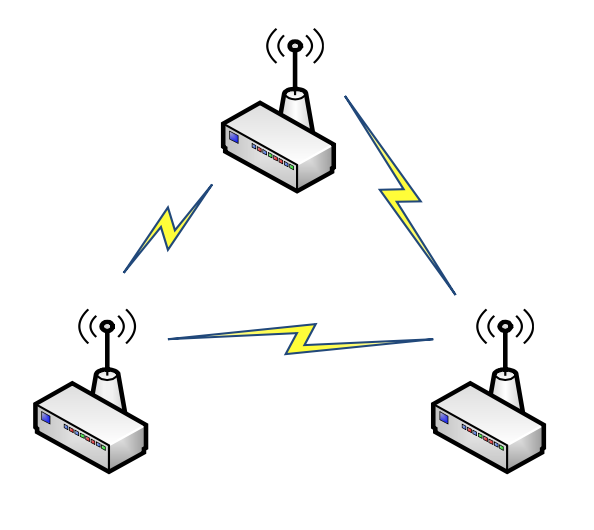
\includegraphics[scale=0.5]{Bilder/peertopeer}
	\caption{Peer-To-Peer Netzwerk\cite{d:kosmerchock}}
	\label{f:peertopeer}
\end{figure}

Bei der Stern-Topologie sind die Sensoren an ein zentrales Kommunikationsgerät angebunden. In diesem Fall kommunizieren die einzelnen Knoten nicht direkt miteinander. Jegliche Art von Kommunikation wird über das zentrale Gerät (auch Hub genannt) geroutet. Der Hub wird hier als Server betrachtet, wohingegen die Knoten (Sensoren) die Clients darstellen. \\

\begin{figure}[H] 
	\centering
	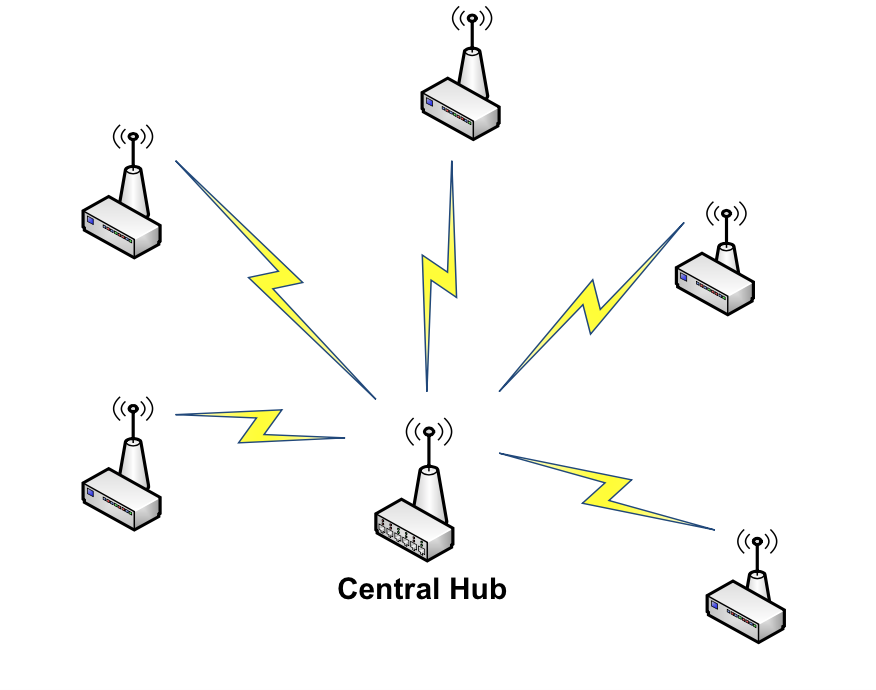
\includegraphics[scale=0.5]{Bilder/star}
	\caption{Stern Netzwerk\cite{d:kosmerchock}}
	\label{f:star}
\end{figure}

Die Baum-Topologie stellt eine Hybridvariante aus Peer-to-Peer und Stern dar. Sie nutzt einen sogenannten 'Root-Knoten' als zentraler Router. Eine Ebene darunter liegen die Hubs, an denen wie in der Stern-Topologie die Sensoren angebunden sind. \\

\begin{figure}[H] 
	\centering
	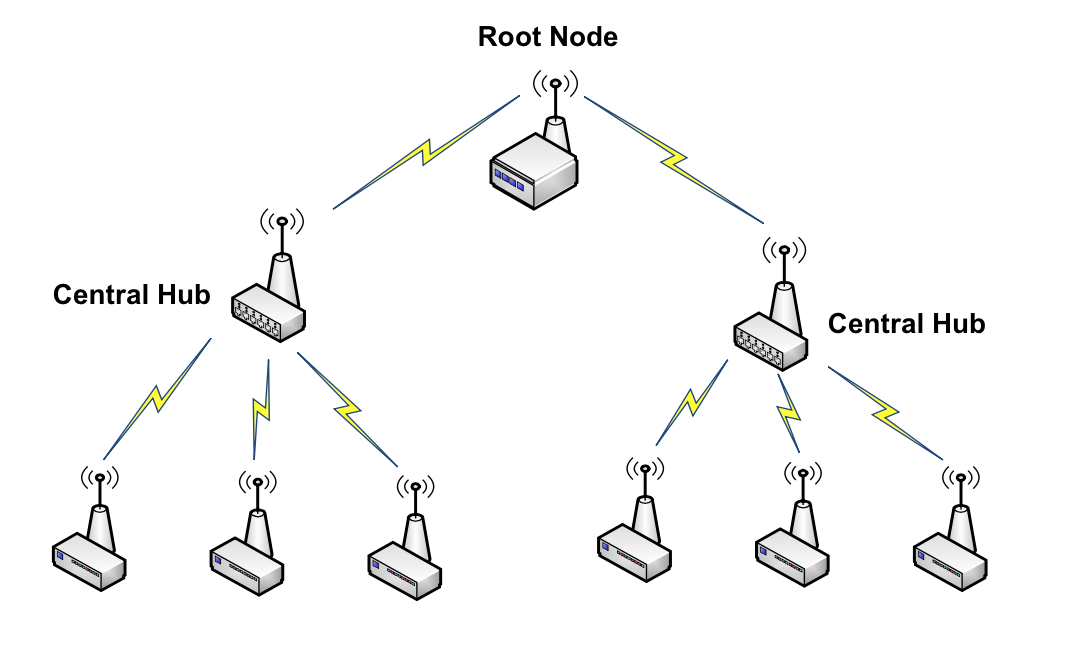
\includegraphics[scale=0.5]{Bilder/tree}
	\caption{Baum Netzwerk\cite{d:kosmerchock}}
	\label{f:tree}
\end{figure}

Eine weitere Mögliche Variante ist ein vermaschtes Netz. Die Knoten sind untereinander ohne zentralen Hub verbunden und die Daten werden einfach von Knoten zu Knoten weitergesendet, bis sie ihr gewünschtes Ziel erreicht haben \cite{d:kosmerchock}. 

\begin{figure}[H] 
	\centering
	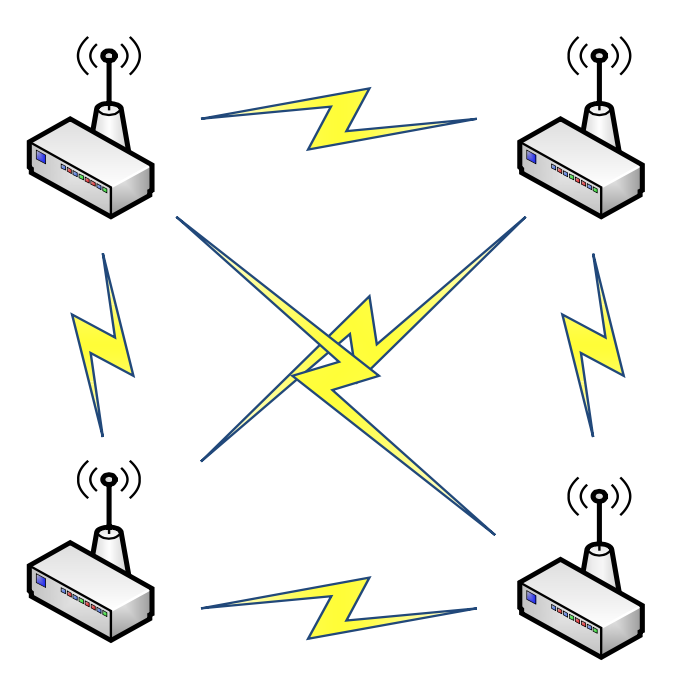
\includegraphics[scale=0.5]{Bilder/mesh}
	\caption{Vermaschtes Netzwerk\cite{d:kosmerchock}}
	\label{f:mesh}
\end{figure}
\subsection{Schwierigkeiten}\label{ss:Schwierigkeiten}

Beim Planen eines drahtlosen Sensornetzwerkes stellen sich vermehrt einige Schwierigkeiten heraus, die zu berücksichtigen sind. Viele dieser Schwierigkeiten sind auch untereinander abhängig und beeinflussen gleichzeitig die verwendete Elektronik, physikalische Aspekte, Rechenleistung oder auch Lebensdauer eines Sensors.\\

Die erste Schwierigkeit, die es bei einem Sensor zu betrachten gilt, ist die Versorgung des Sensors mit Energie. Dazu gibt es unterschiedliche Ansätze, wie z.B. die Versorgung des Sensors mit Batterien. Dies hat allerdings den Nachteil, dass deren Lebenszyklus beschränkt ist und Batterien früher oder später ausgetauscht werden müssen. Ein Akkumulator eignet sich hier besser, allerdings bleibt die Frage, wie der Akkumulator mit neuem Strom versorgt werden soll.\\

In Zusammenhang mit dieser Fragestellung ist die Betrachtung der möglichen Gewinnung oder Rückgewinnung von Energie durch den Sensor von Vorteil. Wie kann ein Sensor Energie gewinnen, ohne dass er damit direkt versorgt werden muss? Möglichkeiten wäre die Gewinnung von Solarenergie durch den Sensor, das Nutzen von Temperaturunterschieden in der Umwelt, die Rückgewinnung der Bewegungsenergie (z.B. durch Wind o.ä.) oder das Ausnutzen von Erschütterungen und Vibrationen. Diese Möglichkeiten sollten nur in Betracht gezogen werden, wenn der Sensor eine lange Lebensdauer mit sich bringen soll. Ist der Einsatz der Sensoren in absehbarer Zeit vorüber, lohnt es sich aus Produktions- und Kostengründen die begrenzte Lebenszeit des Sensors hinzunehmen, um ihn danach z.B. durch neue Sensoren auszutauschen.\\

Ein weiterer wichtiger Aspekt im Bereich Energie ist die Energieeffizienz. Dabei sollen alle Teile in einem Sensorknoten möglichst effizient arbeiten, um die Energie sinnvoll und langsam aufzubrauchen. Nicht nur der Sensor selbst spielt dabei eine wichtige Rolle, sondern auch wie das Netzwerk um ihn herum aufgebaut und genutzt wird. Folgende Aspekte spielen bei der Energieeffizienz eine erhebliche Rolle:

\begin{itemize}
	\item Wahrnehmen der Daten durch die Sensoren
	\item Verarbeitung der Daten
	\item Sicherung der Daten
	\item Übertragung der Daten
	\item Empfang von Daten
\end{itemize} 
\newpage
Damit der Energieverbrauch weiter eingeschränkt werden kann, sollten Sensoren nur aktiv sein, wenn sie wirklich benötigt werden. Ansonsten sollten sie sich in einen Sleep- bzw. Energiesparmodus begeben, um Energie zu sparen. Des Weiteren wäre zur ausschließlichen Wahrnehmung der Umgebung ein 'Controller'- bzw. Sensormodus und zum Senden und Empfangen von Daten ein 'Radio'- bzw. Übertragungsmodus von Vorteil.\\

Eine weitere Schwierigkeit, die sich stellt, ist der Einsatz bzw. die Verteilung der Sensoren in der Umwelt und ihre Selbstverwaltung. Die Knoten könnten entweder zufällig in der Umgebung platziert oder systematisch angeordnet werden. Hier entscheidet der jeweilige Anwendungszweck, wobei das systematische Platzieren der Sensoren meistens sinnvoller und effizienter ist.
Des Weiteren sollte unterschieden werden, ob aktive oder passive Sensoren eingesetzt werden sollen. Auch hier muss je nach Anwendungsfall unterschieden werden. Passive Sensoren eignen sich besser, wenn Daten nur erfasst und übermittelt werden sollen. Aktive Sensoren sollten eingesetzt werden, wenn auf die Erfassung der Daten eine eventuelle Aktion bzw. Reaktion mit der Umwelt erforderlich ist.\\ 

Sensoren sollten bestimmte Informationen über sich selbst und ihre Nachbarn wissen bzw. ermitteln können. Dazu gehören unter anderem ihre eigene Position, die Ortung der Nachbarknoten und ihre Identifikation, ihre eigene Knotenkonfiguration und ihre kürzeste Route zu einer Basisstation. Denn sobald ein Sensornetz einmal in Betrieb genommen wurde, muss es in der Lage sein, sich autonom betreiben und verwalten zu können. Dazu zählen die Anpassung an veränderte Umweltbedingung und das Kompensieren von Fehlern. Beim Ausfall eines einzelnen Sensors soll das Sensornetz weiterhin aktiv und funktionsfähig bleiben.\\

Auch in Hinsicht auf die Sicherheit gibt es einige Aspekte zu betrachten. Manche Sensornetzwerke übertragen empfindliche und kritische Informationen, was sie zu einem beliebten Angriffsziel macht. Sie können sowohl von innen, von außen als auch direkt an den Knoten angegriffen werden. Es stellt sich als schwierig heraus, solche Netzwerke vor Angriffen zu schützen, da sie entfernt und selbstständig arbeiten, drahtlos kommunizieren und meistens keine speziellen Sicherheitsfeatures besitzen. Dies ist aus Energie-, Kostengründen und Gründen der Form und Größe der Sensoren meist nicht realisierbar. Übliche Sicherheitstechniken sind meist nicht durchführbar, da den Knoten üblicherweise die Rechen-, Kommunikations- und Speicherressourcen fehlen. Man braucht neu entwickelte Sicherheitsmechanismen für Sensornetze, die spezielle Lösungen für die Erkennung von Eindringlingen, Verschlüsselung, Schlüsselverwaltung und Verteilung und Registrierung von neuen Knoten besitzen, sodass die Ressourcen der Sensoren ausreichen und das Sicherheitskonzept realisierbar ist \cite{d:wolf}.
\section{Adhoc-Netzwerke}\label{s:AdhocNetzwerke}

Adhoc-Netze sind in sich geschlossene Netzwerke, organisieren sich selbst und haben keine bestimmte Hierarchie. Sie bauen sich nur für die Dauer einer Datenübertragung auf, besitzen keine festgelegte Kommunikationsstruktur und verwalten und organiseren sich selbst. 

Adhoc-Netze sind leistungsfähige und zählen als so genanntes 'Self Organized Network' (SON), welche gute Lastverteilung betreiben und ohne zentrales Management auskommen. Die Endgeräte übernehmen in diesem Fall das Routing und speichern die Routingtabellen selbst ab. Geräte, die sich dem Netzwerk anschließen, werden dynamisch in das Netz eingefügt. Bei Netzwerken nach IEEE 802.11 (WLANs) und IEEE 802.15 (WPANs - hier im Speziellen IEEE 802.15.1 - Bluetooth) werden alle Geräte selbstständig erkannt und werden dem Netz hinzugefügt. Sie sind fortan Bestandteil des Gesamtnetzes. 

Bei Adhoc-Netzen mit vielen Geräten (das kann z.B. ein Sensornetz sein) wird zumeist eine Multihop-Verbindung bevorzugt. Das bedeutet, dass die Daten von einem Netzknoten, z.B. einem Sensor oder Rechner, zu dem nächsten Netzknoten weitergeleitet werden, bis es sein Ziel erreicht hat. Fällt ein Knoten aus, wird wenn möglich ein anderer Weg für die Übertragung genutzt, um Ausfälle zu vermeiden.

Ad-hoc-Netzwerke bestehen virtuell für einen begrenzten Zeitrahmen. Ad-hoc bedeutet etwa "für den Augenblick gemacht". Sie werden in WLANs, WPANs, in Sensornetzen (WPANs mit geringer Datenrate - siehe IEEE 802.15.4) und in Funknetzen von Rettungsdiensten, Polizei und Militär benutzt \cite{ws:lipinski}.

\subsection{MANETs}\label{ss:MANETs}

MANET bezeichnet die Abkürzung für den Begriff 'Mobile Ad-hoc Network‘. Jochen Schiller beschreibt in seiner Literatur 'Mobile Communications' den Begriff des MANETs wie folgt:
 
\begin{quote}
„Ad-hoc-Netze kommen ohne jegliche Infrastruktur aus, insbesondere ohne eine ausgezeichnete Basisstation, welche den Medienzugriff zentral steuert. Diese Netzvariante erlaubt die spontane, nicht vorab geplante Kommunikation zwischen mobilen Endgeräten, wobei einige oder alle Endgeräte auch Daten von anderen Endgeräten weiterleiten können.“
\end{quote}
	
\begin{figure}[H] 
	\centering
	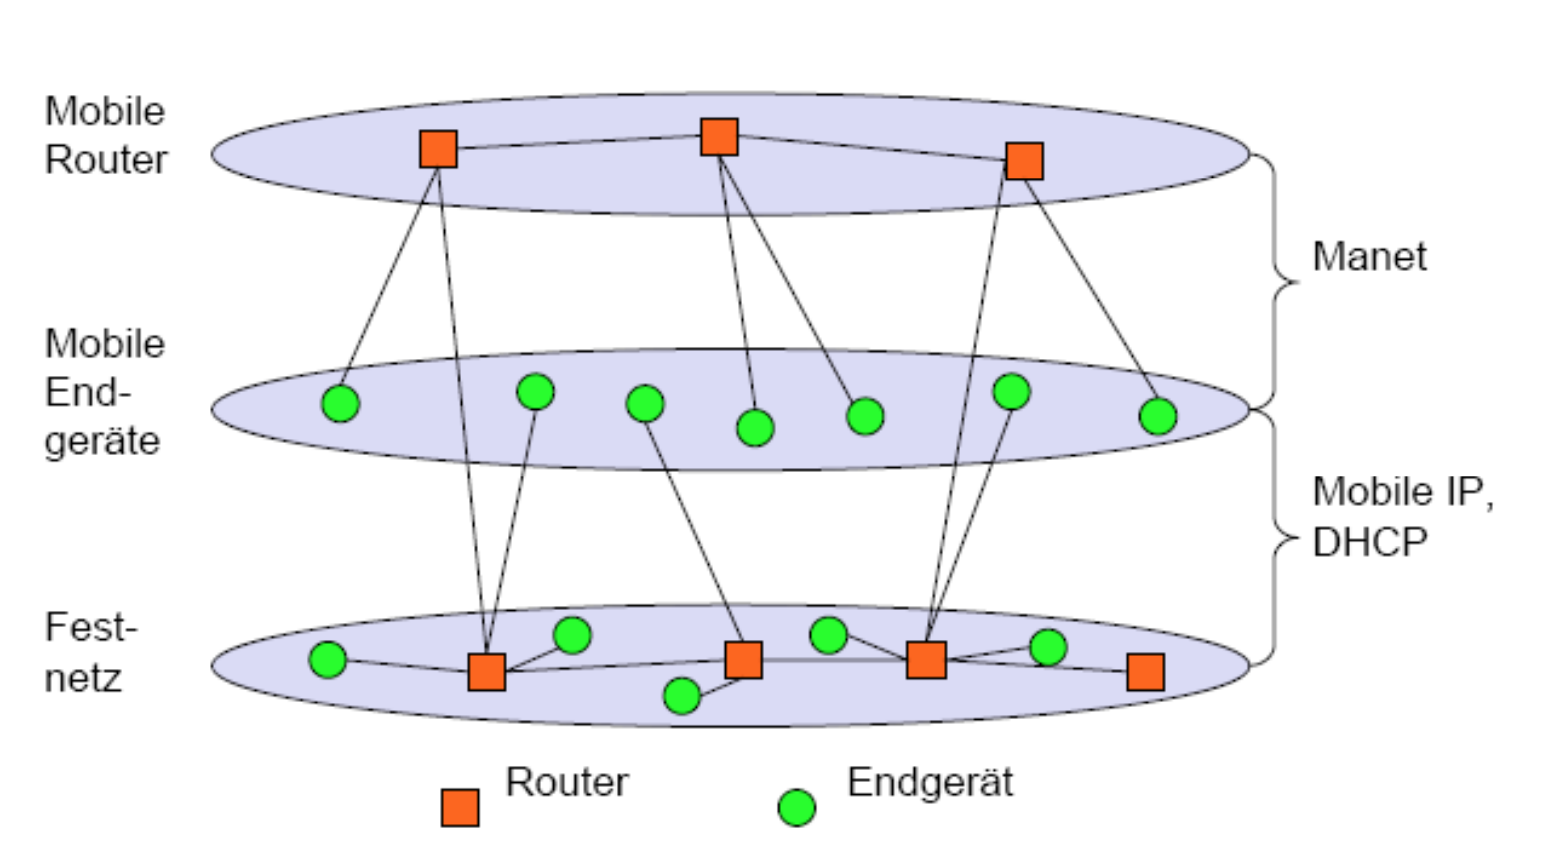
\includegraphics[scale=0.5]{Bilder/manet}
	\caption{Einordnung von MANETs\cite{d:timm}}
	\label{f:manet}
\end{figure}

MANETs zeichnen sich vor allem dadurch aus, dass sie keine feste Infrastruktur besitzen. Es herrscht innerhalb des Netzes eine dynamische Topologie, was bedeutet, dass zu jedem Zeitpunkt bestimmte Knoten wegfallen und neue dazukommen können. Dies führt dazu, dass bislang bekannte und zulässige Routen wegfallen, dafür aber auch neue Routen entstehen können. Unter den Geräten besteht eine spontane Vernetzung. Das bedeutet, dass jedes Gerät sowohl Endpunkt einer Übertragung sein kann, jedoch auch in der Lage sein muss, Daten weiterleiten zu können. Durch dieses Weiterleiten von Daten entsteht eine so genannte 'Multihop-Umgebung‘, da die Daten nicht vom Sender direkt zum Empfänger gelangen, sondern den Empfänger über mehrere Zwischenstationen erreichen. \\

\begin{figure}[H] 
	\centering
	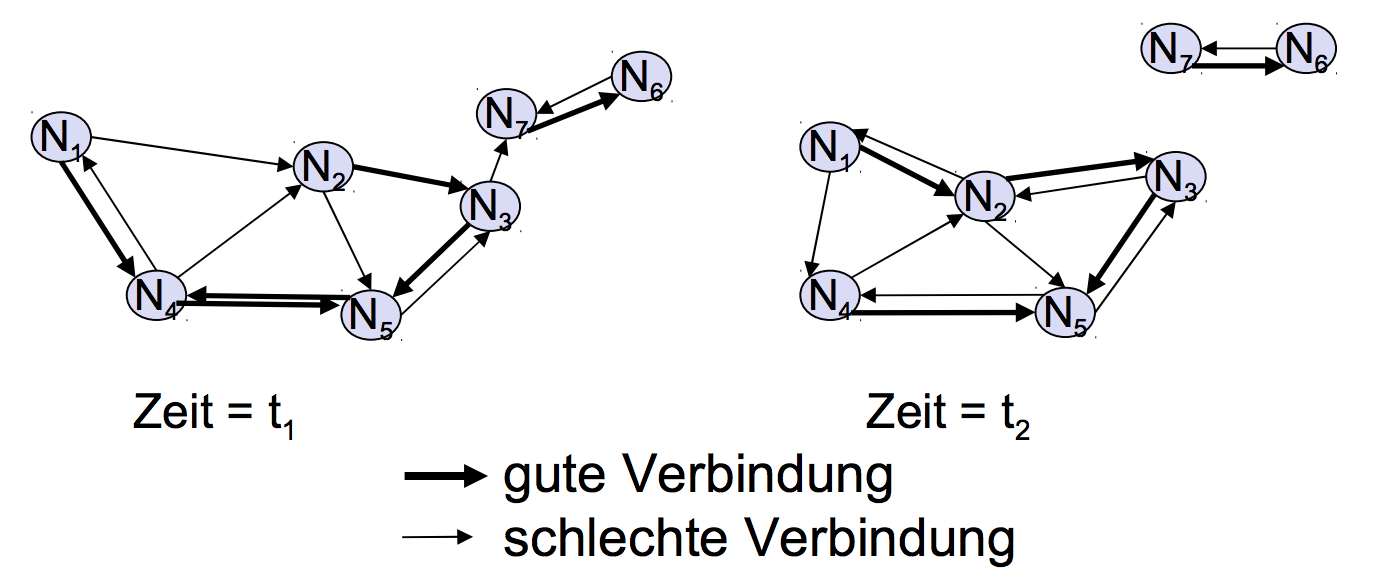
\includegraphics[scale=0.5]{Bilder/manetconnection}
	\caption{Mögliche Verbindungen eines Beispiel MANETs\cite{d:timm}}
	\label{f:manetconnection}
\end{figure}

Mobile Ad-hoc Netzwerke besitzen eine stark begrenzte Bandbreite. Da sie meistens auf stromsparende Übertragungsprotokolle setzen, können dementsprechend auch nur geringe Mengen an Daten übertragen werden. Des Weiteren bestehen zumeist durch die unterschiedlichen Übertragungsleistungen der Geräte asymmetrische Verbindungen, welche sich für die Übertragung von Daten innerhalb des Netzes besser eignen.\\

Ein Problem bei MANETs stellt die beschränkte Möglichkeit der Energieversorgung dar, da die Endgeräte meistens abhängig von Batterien oder Akkus sind. Durch die hohe Menge an Geräten in einem Netz steigt dazu die Summe des potenziellen Energiebedarfes pro Gerät weiter an. Auch die Sicherung des Netzes vor physischen Angriffen ist stark beschränkt. So sind z.B. Denial-of-Service-Attacken (DoS), Überwachungsangriffe oder auch das Verfälschen von Nachrichten oft leicht zu realisieren \cite{d:timm}.

\subsection{Routingprotokolle}\label{ss:Routingprotokolle}

Klassische Routingprotokolle versagen bei dem Versuch, sie innerhalb von mobilen Ad-hoc Netzwerken einzusetzen. Gründe dafür sind folgende: \\

MANETs zeichnen sich durch eine hohe Dynamik aus, das Netz verändert sich spontan, schnell und ständig. Klassische Protokolle besitzen eine zu langsame Konvergenz, um dem Anspruch der sich ständig verändernden Ad-hoc Netze gerecht zu werden und sind somit nicht geeignet.\\

Ad-hoc Netze besitzen wie bereits erwähnt meist eine geringe Bandbreite. Hinzu kommt, dass den angeschlossenen Knoten und Geräten nur eine gewisse Rechenleistung zur Verfügung steht. Sie sind somit mit klassischen Routingprotokollen überfordert, da diese meist viel Rechenleistung und Übertragungsleistung erfordern, welche mit den mobilen Geräten nicht realisierbar sind. Der Overhead der klassischen Protokolle ist also für diese Art von Netzwerken zu groß. \\

Es gibt in mobilen Ad-hoc Netzen gewisse Metriken, die beim Betrieb berücksichtigt werden müssen. Die klassischen Protokolle interessieren sich nicht für diese Metriken und lassen sie außen vor. Bei der Auswahl von Routen müssen unter anderem folgende Aspekte betrachtet werden:
\begin{itemize}
	\item Batterielaufzeit der Geräte
	\item Zeit der Verbindung zwischen zwei Geräten
	\item Energiebedarf
	\item Zuverlässigkeit der Verbindung
\end{itemize} 

Zusammengefasst lässt sich sagen, dass Routingprotokolle für MANETs vor allem eine große Skalierbarkeit im Hinsicht auf eine große Anzahl von Geräten, Flexibilität und Effizienz im Hinblick auf Komplexität, Energieverbrauch und Speicherverbrauch erfordern. Diese werden mittlerweile intensiv erforscht, da Ad-hoc Netze im Zusammenhang mit dem 'Internet of Things‘ (IoT) oder auch dem 'Internet Of Everything‘ (IoE) zunehmend an Bedeutung gewinnen \cite{d:timm}. \\

Im Folgenden sollen die Protokolle OLSR, AODV und CGSR kurz aufgezeigt und erklärt werden.

\subsubsection{OLSR}\label{ss:OLSR}

Die Abkürzung OLSR steht für 'Optimized Link State Routing‘ und bezeichnet ein flaches, proaktives Linkstate-Protokoll. Proaktiv bedeutet in diesem Fall, dass in gewissen Zeitabständen automatisch Kontrollnachrichten ausgetauscht werden. Bei einem Linkstate-Protokoll sendet z.B. jeder Router den anderen Knoten im Netz den Zustand der Verbindung zu seinen Nachbarn. \\
Das OLSR-Routingprotokoll ist als RFC 3626 spezifiziert und erweitert normale Link-State-Protokolle, in dem die Komplexität jener Protokolle vereinfacht wird. \\
Bei OLSR hat jeder Knoten einen Überblick über alle andere Knoten im Netzwerk und den Routen dort hin, somit kann jeder Knoten seine Routen mit dem 'Shortest Path Algorithm‘ eigenständig errechnen. Allerdings haben nicht alle Knoten die gleichen Bedeutungen und Aufgaben.\\
Um Nachbarknoten zu finden, werden sie mit einer 'Hello-Message‘ gesucht. Die Kontrollpakete werden in entsprechenden Zeitabständen erstellt und enthalten die Knotenadresse, eine Sequenznummer und die Nachbarknoten mit Distanzinformationen. Folglich enthält jeder Knoten die Distanzinformationen von allen anderen Knoten, so kann die Topologie erstellt und die Routen mit o.g. 'Shortest Path Algorithm‘ berechnet werden. \\

Das OLSR unterscheidet sich von anderen Link-State-Algorithmen, da es ein optimiertest Link-State-Routing verwendet. Es werden so genannte 'Multi-Point-Relays‘ ausgewählt und verteilt, was für ein effizienteres Routing sorgt. Die Relays sind im Stande, die Kontrollnachrichten an die angeschlossenen Knoten weiterzuleiten.

\begin{figure}[H] 
	\centering
	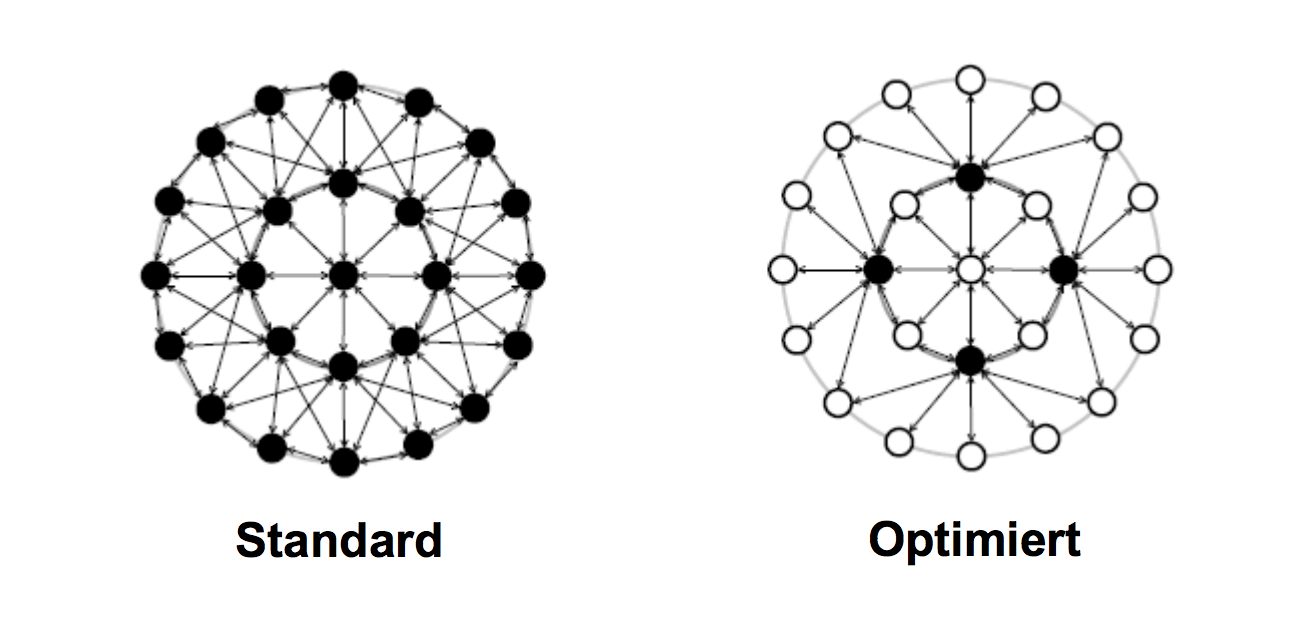
\includegraphics[scale=0.5]{Bilder/olsr}
	\caption{optimiertes LSR durch Multi-Point-Relays im OLSR\cite{d:timm}}
	\label{f:olsr}
\end{figure}

\subsubsection{AODV}\label{ss:AODV}

Das Ad-hoc On-Demand Distance Vector Routingprotokoll ist ein flaches, reaktives Distanzvektorprotokoll. Reaktive Protokolle tauschen im Gegensatz zu proaktiven Protokollen nur Kontrollnachrichten aus, wenn neue Routen benutzt werden sollen. Sie benötigen weniger Bandbreite und sind dynamischer, allerdings besteht nur eine Teilkenntnis des Netzwerks, somit müssen die Routen anders berechnet werden.\\
AODV ist in RFC 3561 spezifiziert und ist für IPv4-Netze vorgesehen. Es erlaubt eine theoretisch unbegrenzte Anzahl von Geräten im Netzwerk. Bei AODV  kennt jeder Knoten nur den 'Next Hop‘, also den nächsten Knoten und die Länge der Gesamtroute. Das Protokoll definiert insgesamt zwei Routingalgorithmen ‚Route Discovery‘ und ‚Route Maintenance‘.  \\

Bei der 'Route Discovery‘ wird die Route aufgebaut, wozu zwei Nachrichtentypen benötigt werden. Es wird zunächst eine 'Route-Request-Nachricht‘ (RREQ) per Broadcast zum Ziel gesendet. Das Ziel antwortet widerum mit einer 'Route-Reply-Nachricht‘ (RREP) per Unicast zurück an den Absender. Sollte eine bidirektionale Verbindung zwischen zwei Geräten herrschen, wird per Route Discovery auch eine bidirektionale Route aufgebaut. \\

\begin{figure}[H] 
	\centering
	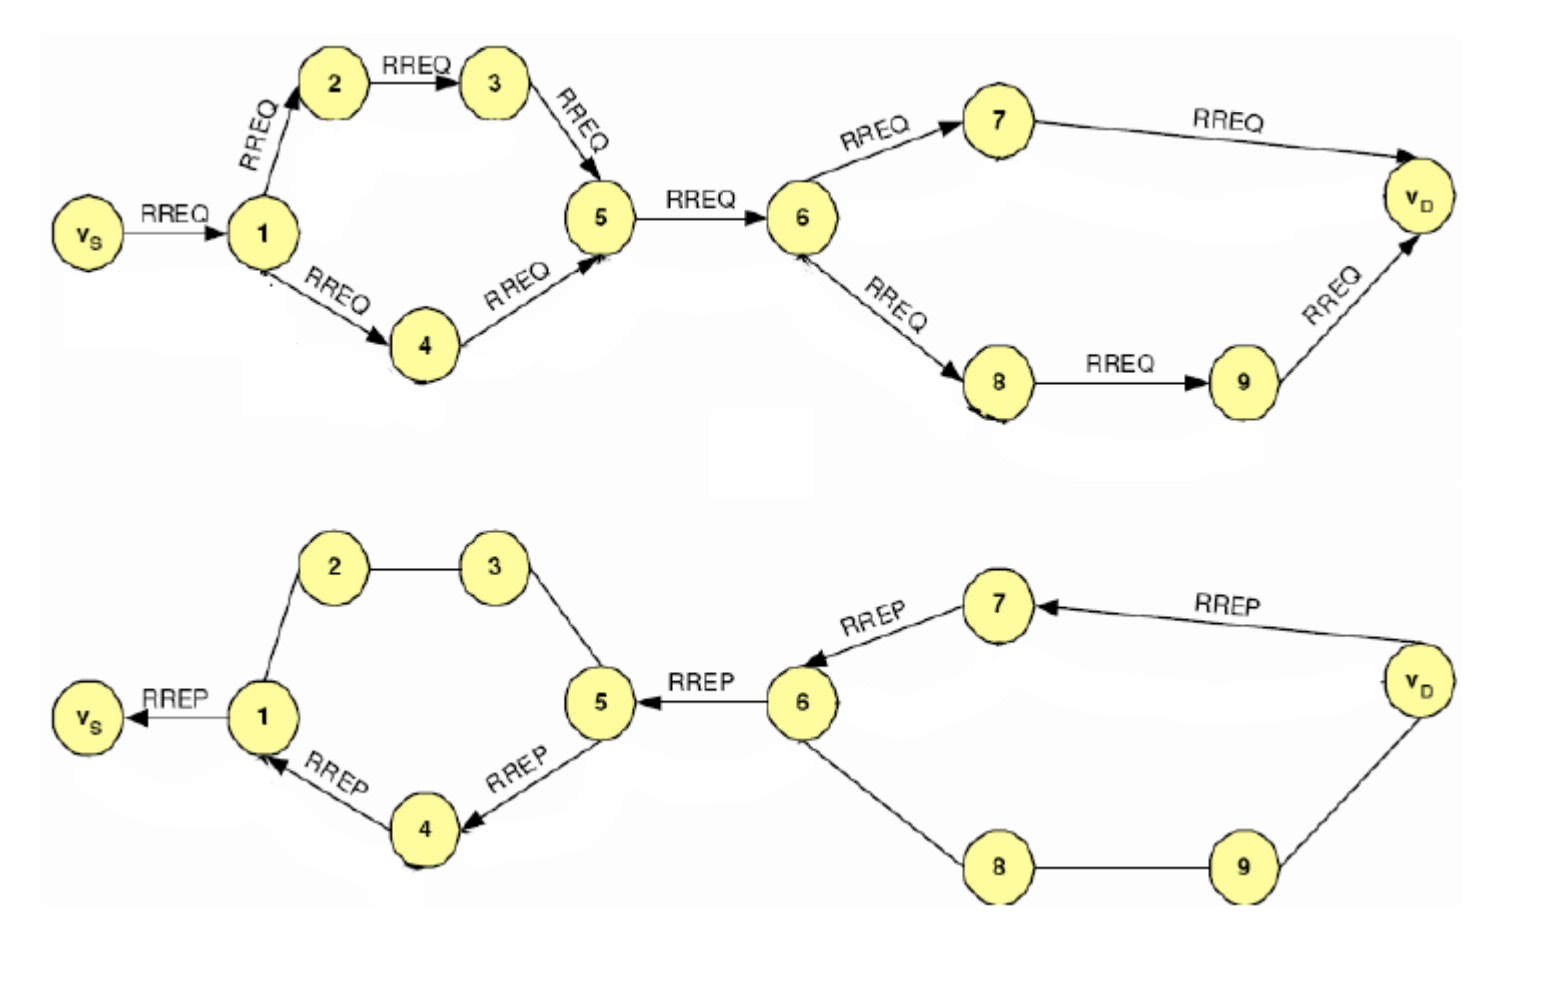
\includegraphics[scale=0.5]{Bilder/aodv}
	\caption{'Route Discovery‘ im AODV-Protokoll\cite{d:timm}}
	\label{f:aodv}
\end{figure}

Bei 'Route Maintenance‘ handelt es sich um die Verwaltung der Routen. Es wird eine 'Route-Error-Nachricht‘ (RRER) versendet, sobald eine defekte Route diagnostiziert wird. Diese Nachricht wird an alle Nachbarn versendet, so dass jeder Knoten über das Wegfallen der Route informiert wird.

\subsubsection{CGSR}\label{ss:CGSR}

Beim Clusterhead-Gateway Switch Routing (CGSR) handelt es sich um ein hierarchisches Protokoll, was bedeutet, dass für verschiedene Knoten unterschiedliche Rollen vorgesehen sind. \\
Das Netzwerk wird bei CGSR in Cluster aufgeteilt, die sich allerdings teilweise überdecken müssen. Für jedes dieser Cluster wird ein 'Clusterhead‘ ernannt. Ein Knoten, welcher sich in zwei Clustern gleichzeitig befindet, wird als Gateway bezeichnet.

\begin{figure}[H] 
	\centering
	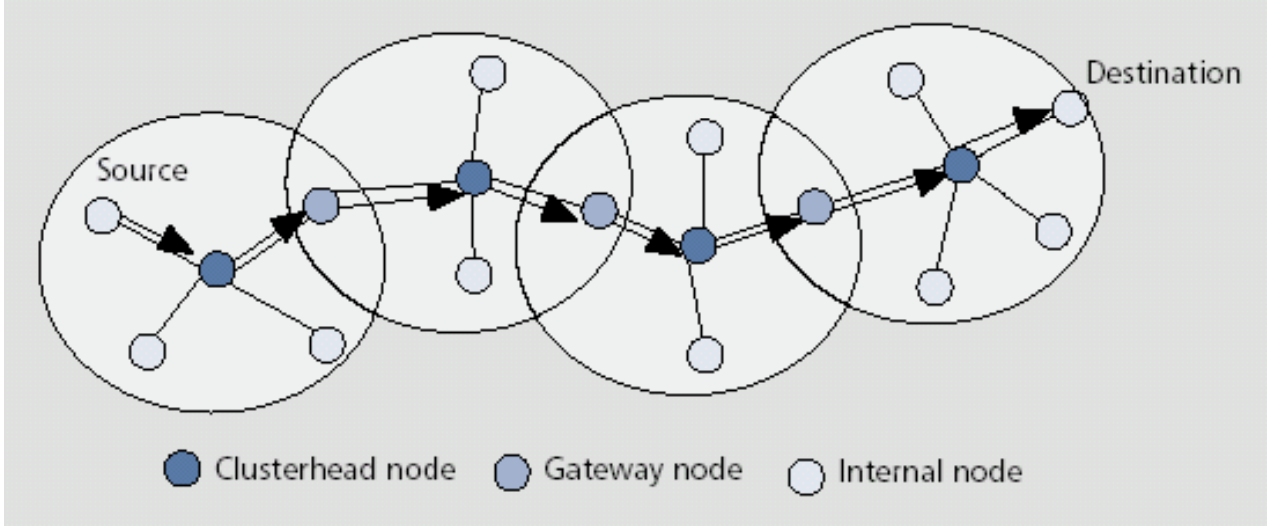
\includegraphics[scale=0.5]{Bilder/cgsr}
	\caption{Clustering im CGSR-Protokoll\cite{d:timm}}
	\label{f:cgsr}
\end{figure}

Das Clusterhead-Gateway Switch Routing basiert auf einem Distanzvektor-Protokoll. Jeder Knoten im Netzwerk speichert sowohl eine Distanzvektor-Routingtabelle, als auch eine 'Cluster Member‘-Tabelle. Die Distanzvektor-Tabelle enthält neben den normalen Routingeinträgen einen Routingeintrag zum Clusterhead jedes Clusters. In der 'Cluster Member‘-Tabelle wird für jeden Knoten der Clusterhead gespeichert, damit klar ist, welcher Knoten zu welchem Cluster gehört. \\

Der große Vorteil von CGSR besteht in der signifikanten Reduzierung der Größe der Routingtabellen im Vergleich zu anderen Distanzvektorprotokollen, somit ist das CGSR für Ad-hoc Netzwerke dank seiner geringeren Komplexität gut geeignet.


\section{IEEE 802.15.4}\label{ss:IEEE802154}

Das ‚Institute of Electrical and Electronics Engineers‘ (IEEE) definiert in seinem Standard 802.15.4 Protokolle für ein ‚Low Data Rate - Wireless Personal Area Network‘ (LR-WPAN). Die Art der Geräte, die für eine solche Art von Netz verwendet werden sollen, ist dabei nicht genauer spezifiziert. Sinnvoll ist der Einsatz vor allem bei Systemen wie Sensoren, Lichtquellen oder Schaltern, bei welchen eine niedrige Datenrate vollkommen ausreicht um miteinander zu kommunizieren. Grundsätzlich ist die Verwendung des Standards auch bei höherwertigen Geräten wie z.B. Handys oder anderen Multimediageräten möglich, allerdings ist die Sinnhaftigkeit eines solchen Einsatzes fragwürdig, da in Hinsicht auf die geringe Datenübertragungsrate viele Übertragungs- und Kommunikationsfunktionen solcher Geräte wohl kaum realisierbar wären. \\
Zur Kommunikation mehrerer Teilnehmer in einem nach 802.15.4-standardisierten Netzes werden die o.g. Topologien ‚Stern‘ und ‚Peer-to-Peer‘ unterstützt. Sollte die Spezifikation ‚ZigBee‘,  welche den 802.15.4 Standard erweitert, verwendet werden, können darüber hinaus auch vermaschte Netze realisiert werden. \\
Der Standard sendet laut Definition festgelegtem Frequenzspektrum auf den lizenzfreien Frequenzen 868-868,8 MHz (Europa), 902-928 MHz (Nordamerika, Australien) oder 2400 bis 2483,5 MHz (weltweit). Um die Frequenzen darüber hinaus zu spreizen, wird ein ‚Direct Sequence Spread Spectrum‘-Verfahren (DSSS) verwendet. //
Um den Zugriff auf das Medium untereinander zu koordinieren, wird CSMA/CA (‚Carrier Sense Multiple Access/Collision Avoidance‘) verwendet. Das bedeutet, dass, bevor ein Gerät mit einer Übertragung beginnt, überprüft wird, ob das Übertragungsmedium nicht bereits von einem anderen Endgerät genutzt wird. Ist das Medium nicht belegt, kann das Endgerät, welches das Medium überprüft hat, anfangen, seine Daten zu übertragen.\\
Der Standard erreicht Übertragungsraten zwischen 20 KB/s - 40 KB/s in den Frequenzbereichen von 868 MHz und 902-928 MHz, wohingegen im 2,4 GHz-Bereich Raten bis zu 250 KB/s realisiert werden können. Diese relativ geringen Datenraten zeigen bereits, dass der Standard nicht für eine Übertragung großer Daten konzipiert wurde. Es soll viel mehr eine energiesparende Übertragung geringer Datenmengen verwirklicht werden können \cite{d:hesse}.

\subsection{Komponenten}\label{ss:Komponenten}

\subsection{Unterstützte Topologien}\label{ss:UnterstutzeTopologien}

\subsection{Schichten}\label{ss:Schichten}

\subsection{Rahmenstruktur}\label{ss:Rahmenstruktur}

\subsection{Kommunikation}\label{ss:Kommunikation}

\subsection{Medienzugriff}\label{ss:Medienzugriff}

\subsection{Sicherheitsma"snahmen}\label{ss:Sicherheitsmassnahmen}
\section{SunSPOT}\label{s:Sunspot}

Die Firma Oracle besitzt im Rahmen seiner Java-Technologie eine Vormachtstellung im Bereich der Smartphones.
Auf der Welt sind schätzungsweise über eine Milliarde Smartphones mit der Java-Technologie lizenziert. \cite{d:horan} \\ Ziel von Oracle ist es, auch in den zukunftsnahen Technologien mit ihrer Programmiersprache Java auszustatten und diese Produkte zu etablieren.\\

Ein erster Schritt in diese Richtung is das von Oracle entwickelte "'SunSPOT"'-Sensornetzwerk. SunSPOT bedeutet "'Sun Small Programmable Object Technology"' und ist eine Plattform für Java-basierte drahtlose Sensornetzwerke. Sie bestätigt den Trend, dass in immer kleiner werdenden Geräten zunehmend leistungsfähigere Technologien eingesetzt werden. Dabei ist wichtig, dass jene Geräte, am Besten drahtlos, miteinander kommunizieren können und jederzeit von überall auf der Welt steuerbar bleiben. Das SunSPOT Starter Paket besteht aus einer Basisstation und 2 Sensoren. \\

\begin{figure}[H] 
	\centering
	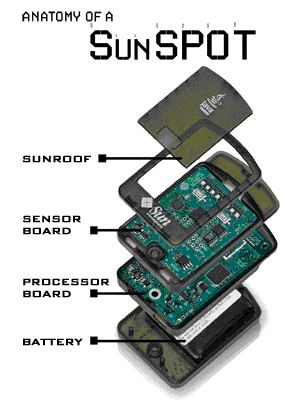
\includegraphics[scale=0.5]{Bilder/spotanatomy}
	\caption{Anatomie eines Standard SunSPOT-Sensors\cite{i:spotaufbau}}
	\label{f:spotaufbau}
\end{figure}

Die Hardware der SunSPOT-Sensoren ist modular aufgebaut. Das bedeutet, dass man die verfügbaren Boards frei nach Belieben aufeinander stecken und somit verbinden kann. Dabei können maximal bis zu 3 Boards + Stromversorgung miteinander verknüpft werden. \cite{d:horan} \\

\subsection{Technische Daten}\label{ss:TechnischeDaten}

Hier werden alle technischen Daten der SunSPOTS erklärt.



\chapter{Praktische Arbeiten mit SunSPOT}\label{c:PraktischeArbeiten}

In diesem Kapitel werden wir die praktischen Arbeiten, die wir mit SunSPOTS durchführen erläutern. Dies wird in zwei Unterkapiteln durchgeführt.

\section{Erste Schritte}\label{s:ErsteSchritte}

Um den Umgang mit den SunSPOTs zu erlernen und ihre Software und Hardware kennen zu lernen, bietet Oracle auf der Website eine Anleitung inklusive Übungen an, welche sukzessive abgearbeitet werden kann. Die Anleitung umfasst die Installation der Software sowie das Ausführen von Testprogrammen, welche die Fähigkeiten des SunSPOTs demonstrieren.

\subsection{Installation}\label{s:Installation}

Zur Installation der Verwaltungsapplikation 'SunSPOT Manager' und dem SunSPOT SDK, mit welchem man die Programm für die SunSPOTs schreibt, startet man das 'SunSPOT Manager Java Webstart' Programm. Das Webstart-Programm lädt darauf hin den Manager und das SDK herunter und installiert es auf der Workstation. Zur einwandfreien Benutzung des Managers müssen folgende Tools vorhanden sein:

\begin{itemize}
	\item ein aktuelles Java Development Kit
	\item Apache ANT
	\item optional: NetBeans IDE
\end{itemize}

Das Installationsprogramm weist auf ein Fehlen oben genannter Tools hin und installiert diese bei Bedarf nach. Sollte dies nicht automatisch durch das Programm geschehen, können diese Programme auch manuell nachinstalliert werden.
Während der Installation wird nach dem SunSPOT SDK gefragt, welches installiert werden soll. Je nach Version der SPOTs ist hier die entsprechende Version auszuwählen.\\

Normalerweise wird beim Anschließen per USB der entsprechende Treiber für die SPOTs automatisch installiert. Bei aktuellen 64-bit Windows-Versionen (7/8/8.1) kommt es allerdings zu Schwierigkeiten. Eine spezielle Treiber-Datei wurde am 7. Mai 2010 durch Bob Alkire im Oracle-Blog veröffentlicht und kann dort heruntergeladen werden. Mit ihr ist es möglich, die SPOTs auch mit aktuellen 64-bit Windows-Plattformen zu verwenden \cite{ws:alkire}.\\

Sobald der Manager und alle zugehörigen Treiber erfolgreich installiert wurden, können Programme mit Hilfe von NetBeans oder einer anderen IDE geschrieben und auf den SPOT übertragen werden.

\subsection{Übung 1 - Flashlight}\label{s:Uebung1}

In der ersten Übung soll das erste Beispielprogramm 'Flashlight' auf den SPOT übertragen, dort ausgeführt und die zugehörigen Programmausgaben (Konsolen- \& Debugausgaben) betrachtet werden. 

Nach dem erfolgreichen Übertragen des Programms blinken die LEDs des SPOTs in kurzem Abstand, vorausgesetzt, es wird ein bestimmter Helligkeitswert, ausgelesen vom Lichtsensor, nicht überschritten. Mit Hilfe des rechten Knopfschalters auf dem Sensorboard kann außerdem die Farbe der LEDs geändert werden. Die Konsolenausgabe des Programms besteht aus dem momentanen Helligkeitswert, der vom Lichtsensor erfasst wird.

\begin{figure}[H] 
	\centering
	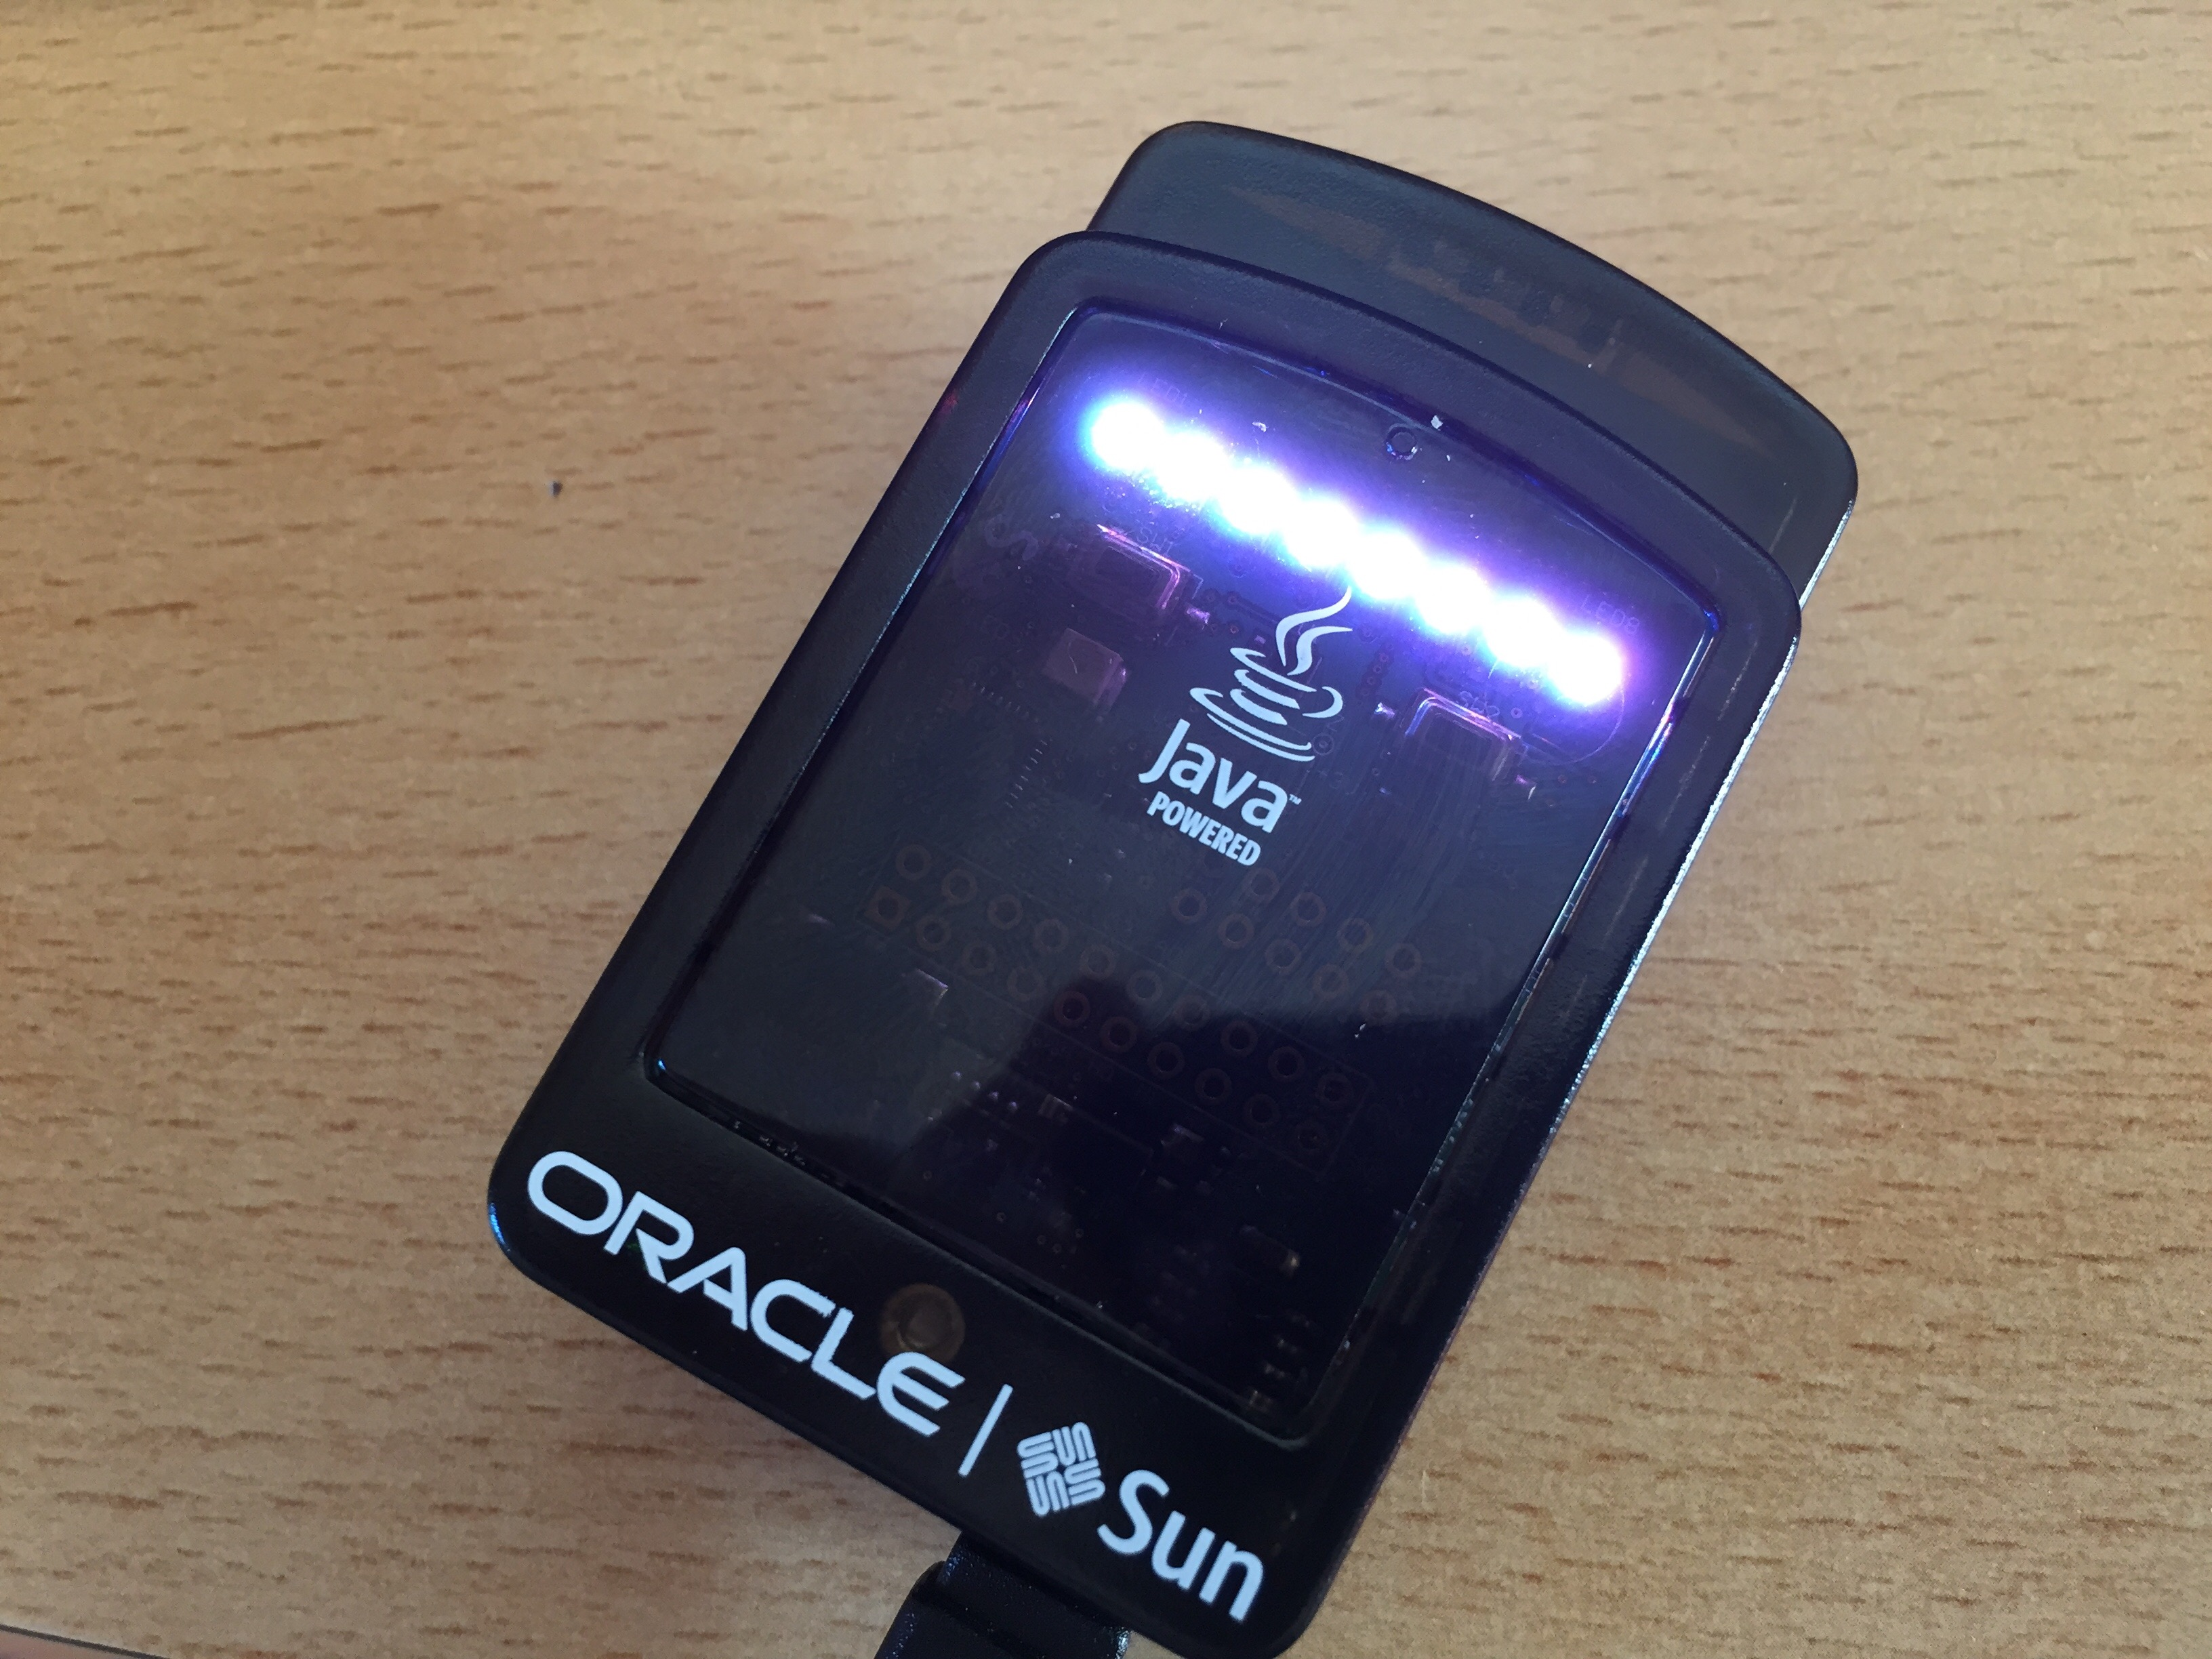
\includegraphics[scale=0.08]{Bilder/uebung1}
	\caption{Leuchtende LEDs des 'Flashlight'-Programms}
	\label{f:uebung1}
\end{figure}

Für die geplante Raumüberwachung ist diese Übung insofern hilfreich, als das hier der Umgang mit den LEDs und deren Verhalten auf äußere Einflüsse gezeigt wurde. In der späteren Implementierungsphase der Raumüberwachung sollen LEDs anzeigen, ob eine Bewegung und somit ein illegales Eindringen in den Raum stattfand.

\section{Implementierung einer Raum\"uberwachung}\label{s:ImplementierungRaumueberwachung}

\subsection{Idee}\label{ss:Idee}

Nicht nur für Museen, Villen oder Betriebe ist ein Sicherheitssystem sinnvoll, denn besonders in private Wohnungen und Häuser wird gerne eingebrochen.

\begin{figure}[H] 
	\centering
	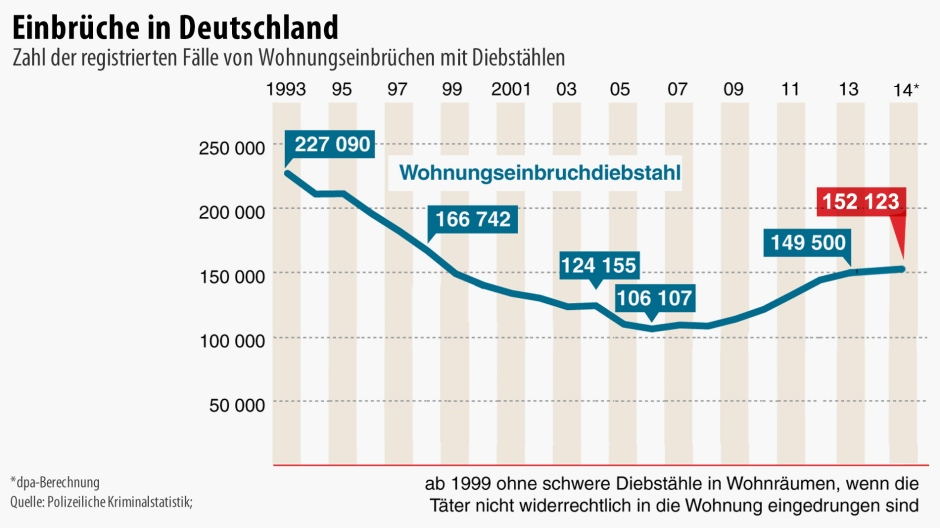
\includegraphics[scale=0.35]{Bilder/einbrueche}
	\caption{Einbruchsstatistik in Deutschland\cite{i:einbrueche}}
	\label{f:einrbrueche}
\end{figure}

Allein im Jahr 2014 wurde über 150.000 mal in Deutschland ein Einbruch mit Diebstahl gemeldet. Die Aufklärungsrate der Verbrechen hingegen ist jedoch sehr gering. Um sich vor solchen Straftaten zu schützen werden Überwachungsanlagen immer beliebter.\\
Im Rahmen dieser Studienarbeit soll eine Raumüberwachung entwickelt werden, die mit Hilfe von untereinander vernetzten Sensoren Einbrüche frühzeitig erkennt, und an den Besitzer meldet. Die Überwachung soll direkt an Fenster und Türen stattfinden, mit Hilfe von Vibrationssensoren, Mikrophonen oder Kameras sollen außergewöhnliche Vorkommnisse ausgewertet werden. Bei einem Einbruch kann dies dem Besitzer über das Netzwerk mitgeteilt werden.


\subsection{Umsetzung}\label{s:Umsetzung}

Im Rahmen der Studienarbeit wurden mit der NetBeans IDE und der Programmiersprache Java zwei Applikationen erstellt, welche einen ersten Ansatz für eine Einbruchsicherung realisieren. Sie sind beliebig erweiterbar, so dass diese als Grundlage für eine komplexere Raumüberwachung dienen können. Die Gesamtimplementation wurde in zwei Teilapplikationen aufgeteilt. Die erste Applikation ist die ‚Desktop-Applikation‘, welche auf dem Rechner läuft und die Daten vom SunSPOT-Sensor empfängt. Auf dem SunSPOT läuft der zweite Teil der Implementation, welcher Bewegungen des Sensors feststellt und diese an eine SunSPOT-Basisstation weiterleitet. In den folgenden Abschnitten wird die genauere Funktionsweise der zwei Teilapplikationen behandelt.

\subsubsection{Desktop-Applikation}\label{sss:Desktop-Applikation}

Die Desktop-Applikation der praktischen Arbeit umfasst knapp 100 Zeilen und dient zum Aufbau einer Radiogram-Verbindung zwischen SunSPOT und Basisstation sowie zum Empfang der vom SPOT gesendeten Daten. 

\begin{lstlisting}[language=Java,caption={Ausschnitt aus der setup()-Methode},label=lst:setup,frame=single] 
private void setup() {
	fr = new JFrame("Einbruchsicherung");
	status = new JTextArea();
	JScrollPane sp = new JScrollPane(status);
	fr.add(sp);
	fr.setSize(360, 200);
	fr.validate();
	fr.setVisible(true);
}           
\end{lstlisting}

Im ersten Schritt wird die Methode ‚setup()‘ definiert, welche zur besseren Visualisierung der Informationen einen JFrame erstellt, in welchen nachher eingetragen werden kann, dass der Sensor eine Bewegung erfahren hat. Sie wird zum Start des Programms aufgerufen, damit das Fenster auch entsprechend erstellt wird. \\

Des weiteren ist eine Methode ‚run()‘ vorhanden, welche direkt nach der ‚setup()‘-Prozedur aufgerufen wird. Diese Funktion kümmert sich sowohl um das Öffnen eines serverseitigen Ports als auch um den Empfang von Datenpaketen, welche an diesen Port versendet werden. \\
Um Daten vom Sensor empfangen zu können, muss in der Desktop-Applikation auf einem selbst festgelegten Port nach Verbindungen ‚gelauscht‘ werden. 
\\
\begin{lstlisting}[language=Java,caption={Öffnen des serverseitigen Ports},label=lst:portserver,frame=single] 
try {
	// Oeffnen einer Radiogram-Verbindung auf der Desktop-Seite
	// um Daten von Sensoren empfangen zu koennen
	rCon = (RadiogramConnection) Connector.open("radiogram://:" + HOST_PORT);
	dg = (Radiogram)
	rCon.newDatagram(rCon.getMaximumLength());
	} 
	
catch (Exception e) {
	System.err.println("setUp caught " + e.getMessage());
	throw e;
}
\end{lstlisting}

Der oben gezeigte Codeausschnitt eröffnet einen serverseitigen Port mit Hilfe der vorher festgelegten HOST\_PORT Variable und lauscht nun fortan auf diesem für Pakete, die vom SunSPOT an die Basisstation versendet werden.\\

\begin{figure}[H] 
	\centering
	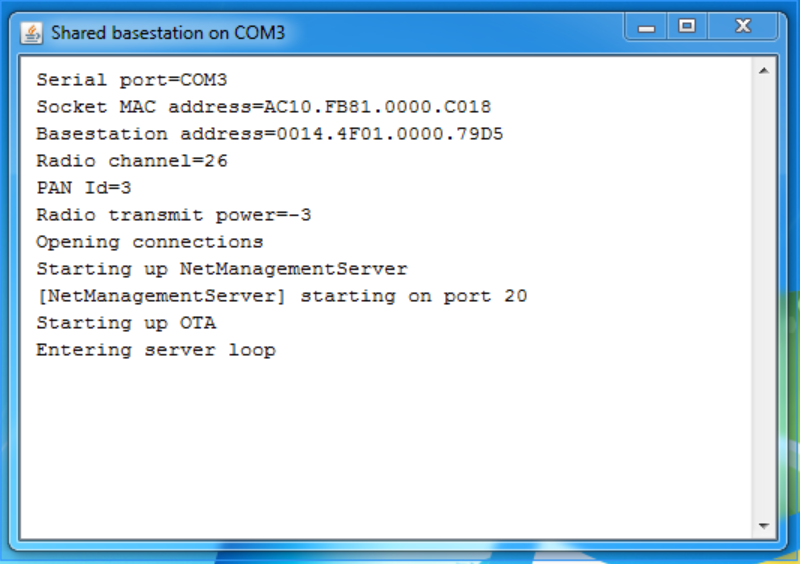
\includegraphics[scale=0.5]{Bilder/server}
	\caption{Logdaten der Basisstation bei Servererstellung}
	\label{f:server}
\end{figure}

Der zweite Teil der ‚run()‘-Methode besteht aus einer while-Schleife, welches auf ankommende Pakete wartet und diese entgegennimmt. Nur wenn der SPOT eine Bewegung erfährt, sendet er ein Paket an die Basisstation. So kann die Desktop-Applikation sicher sein, dass immer, wenn ein Paket gesendet wird, eine Bewegung stattfand.\\

\begin{lstlisting}[language=Java,caption={Auswerten des empfangenen Paketes},label=lst:rcvpackage,frame=single] 
while (true) {
	try {
		// Empfangen und Lesen des Pakets
		rCon.receive(dg);
		long time = dg.readLong();
		System.out.println(time);
		status.append("Bewegung festgestellt!\n");
		} 
	catch (Exception e) {
		System.err.println("Exception " + e +  " beim Lesen der Daten.");
		throw e;
		}
	}
\end{lstlisting}

Innerhalb des übermittelten Paketes befindet sich die aktuelle Uhrzeit, um die Bewegung nachher genau zeitlich einordnen zu können. Sobald die Desktop-Applikation ein Paket empfängt, gibt sie auf dem Bildschirm innerhalb des erstellten Frames den Text 'Bewegung festgestellt!' aus. So wird dem Nutzer unmissverständlich klar gemacht, dass der Sensor in Bewegung war.

\begin{figure}[H] 
	\centering
	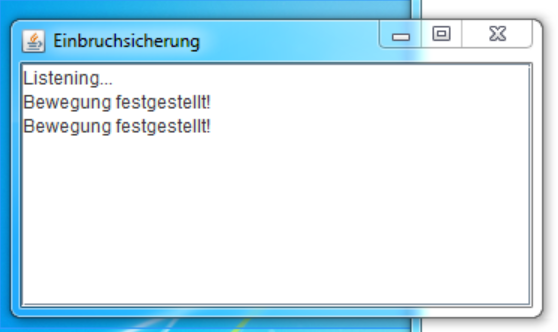
\includegraphics[scale=0.8]{Bilder/bewegung}
	\caption{JFrame mit textueller Ausgabe}
	\label{f:bewegung}
\end{figure}

Innerhalb der Konsole werden neben Debugausgaben zur Basisstation und die Liste eröffneter Ports der Zeitstempel, welcher mit der Bewegung vom SunSPOT übermittelt wird, ausgegeben.

\begin{figure}[H] 
	\centering
	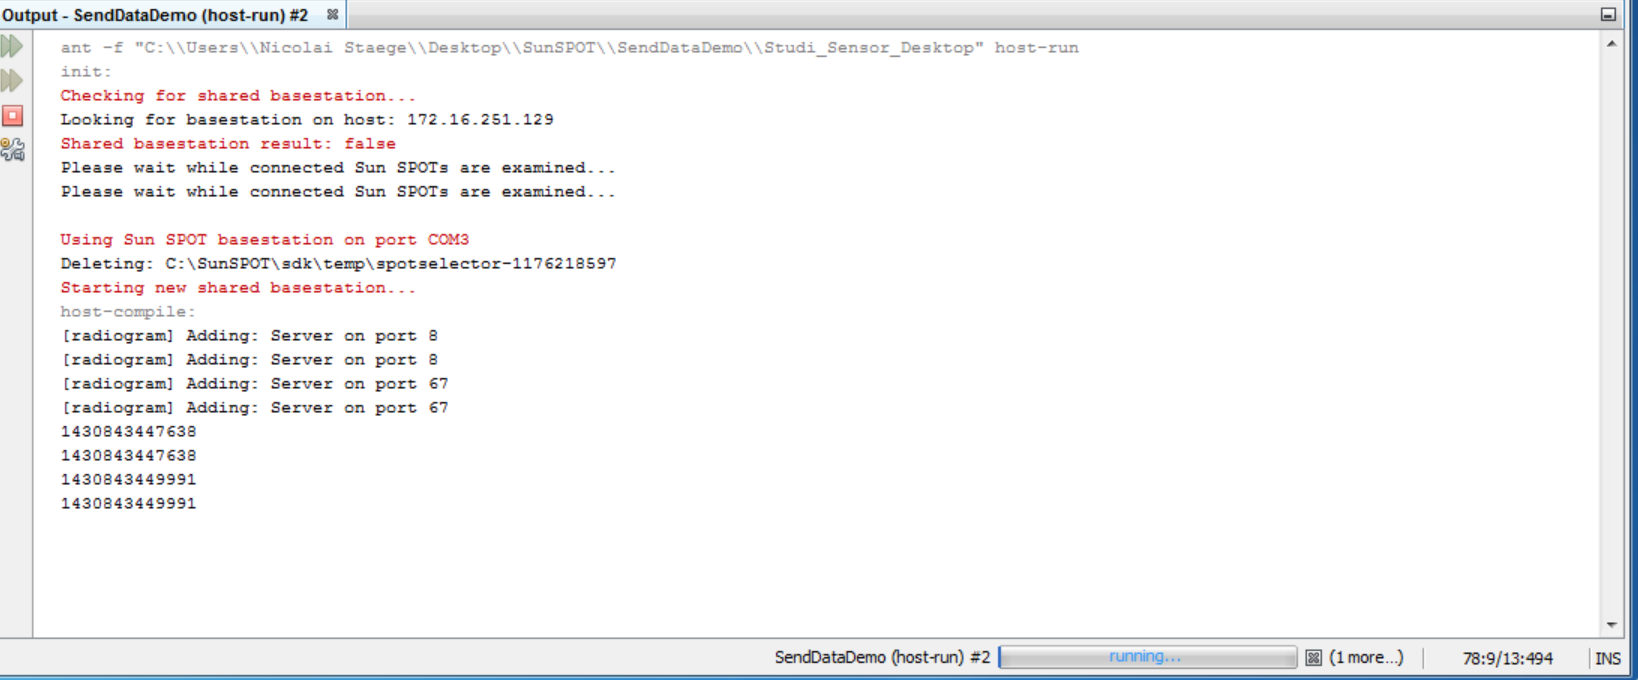
\includegraphics[scale=0.5]{Bilder/timestamp}
	\caption{Konsolenausgabe mit Timestamp}
	\label{f:timestamp}
\end{figure}

\subsubsection{SPOT-Applikation}\label{sss:SPOT-Applikation}

\chapter{Vergleichbare Projekte}\label{c:VergleichbareProjekte}

\section{Smart Greenhouse}\label{s:SmartGreenhouse}

Das Projekt Smart Greenhouse ist die das im folgenden Kapitel \myref{s:Bot-So} beschriebene Projekt ein Gewinner der Kategorie "professional", der IoT Developer Challenge. 
Der Begriff Smart Greenhouse steht für eine \ac{IoT}-Komponente und Applikation, mit der ein Gewächshaus überwacht und kontrolliert werden kann. Das Konzept hierfür entstand, als das Team, bestehend aus Dzmitry Yasevich, Pavel Vervenko und Vladimir Redzhepov, die JavaOne-Messe Russland im April 2013 besuchten. Die Gründer des Projekts sahen dort eine Präsentation eines Intelligenten Hauses, das mithilfe verschiedener Roboter und weiteren durch Java betriebene vernetzte Geräten viele Komfortfunktionen für Bewohner bereitstellte. "Wir waren beeindruckt und hatten eine Idee, etwas ähnliches wie das zu entwickeln vgl. \cite{z:smartgreenhouse}."

\begin{figure}[H] 
	\centering
	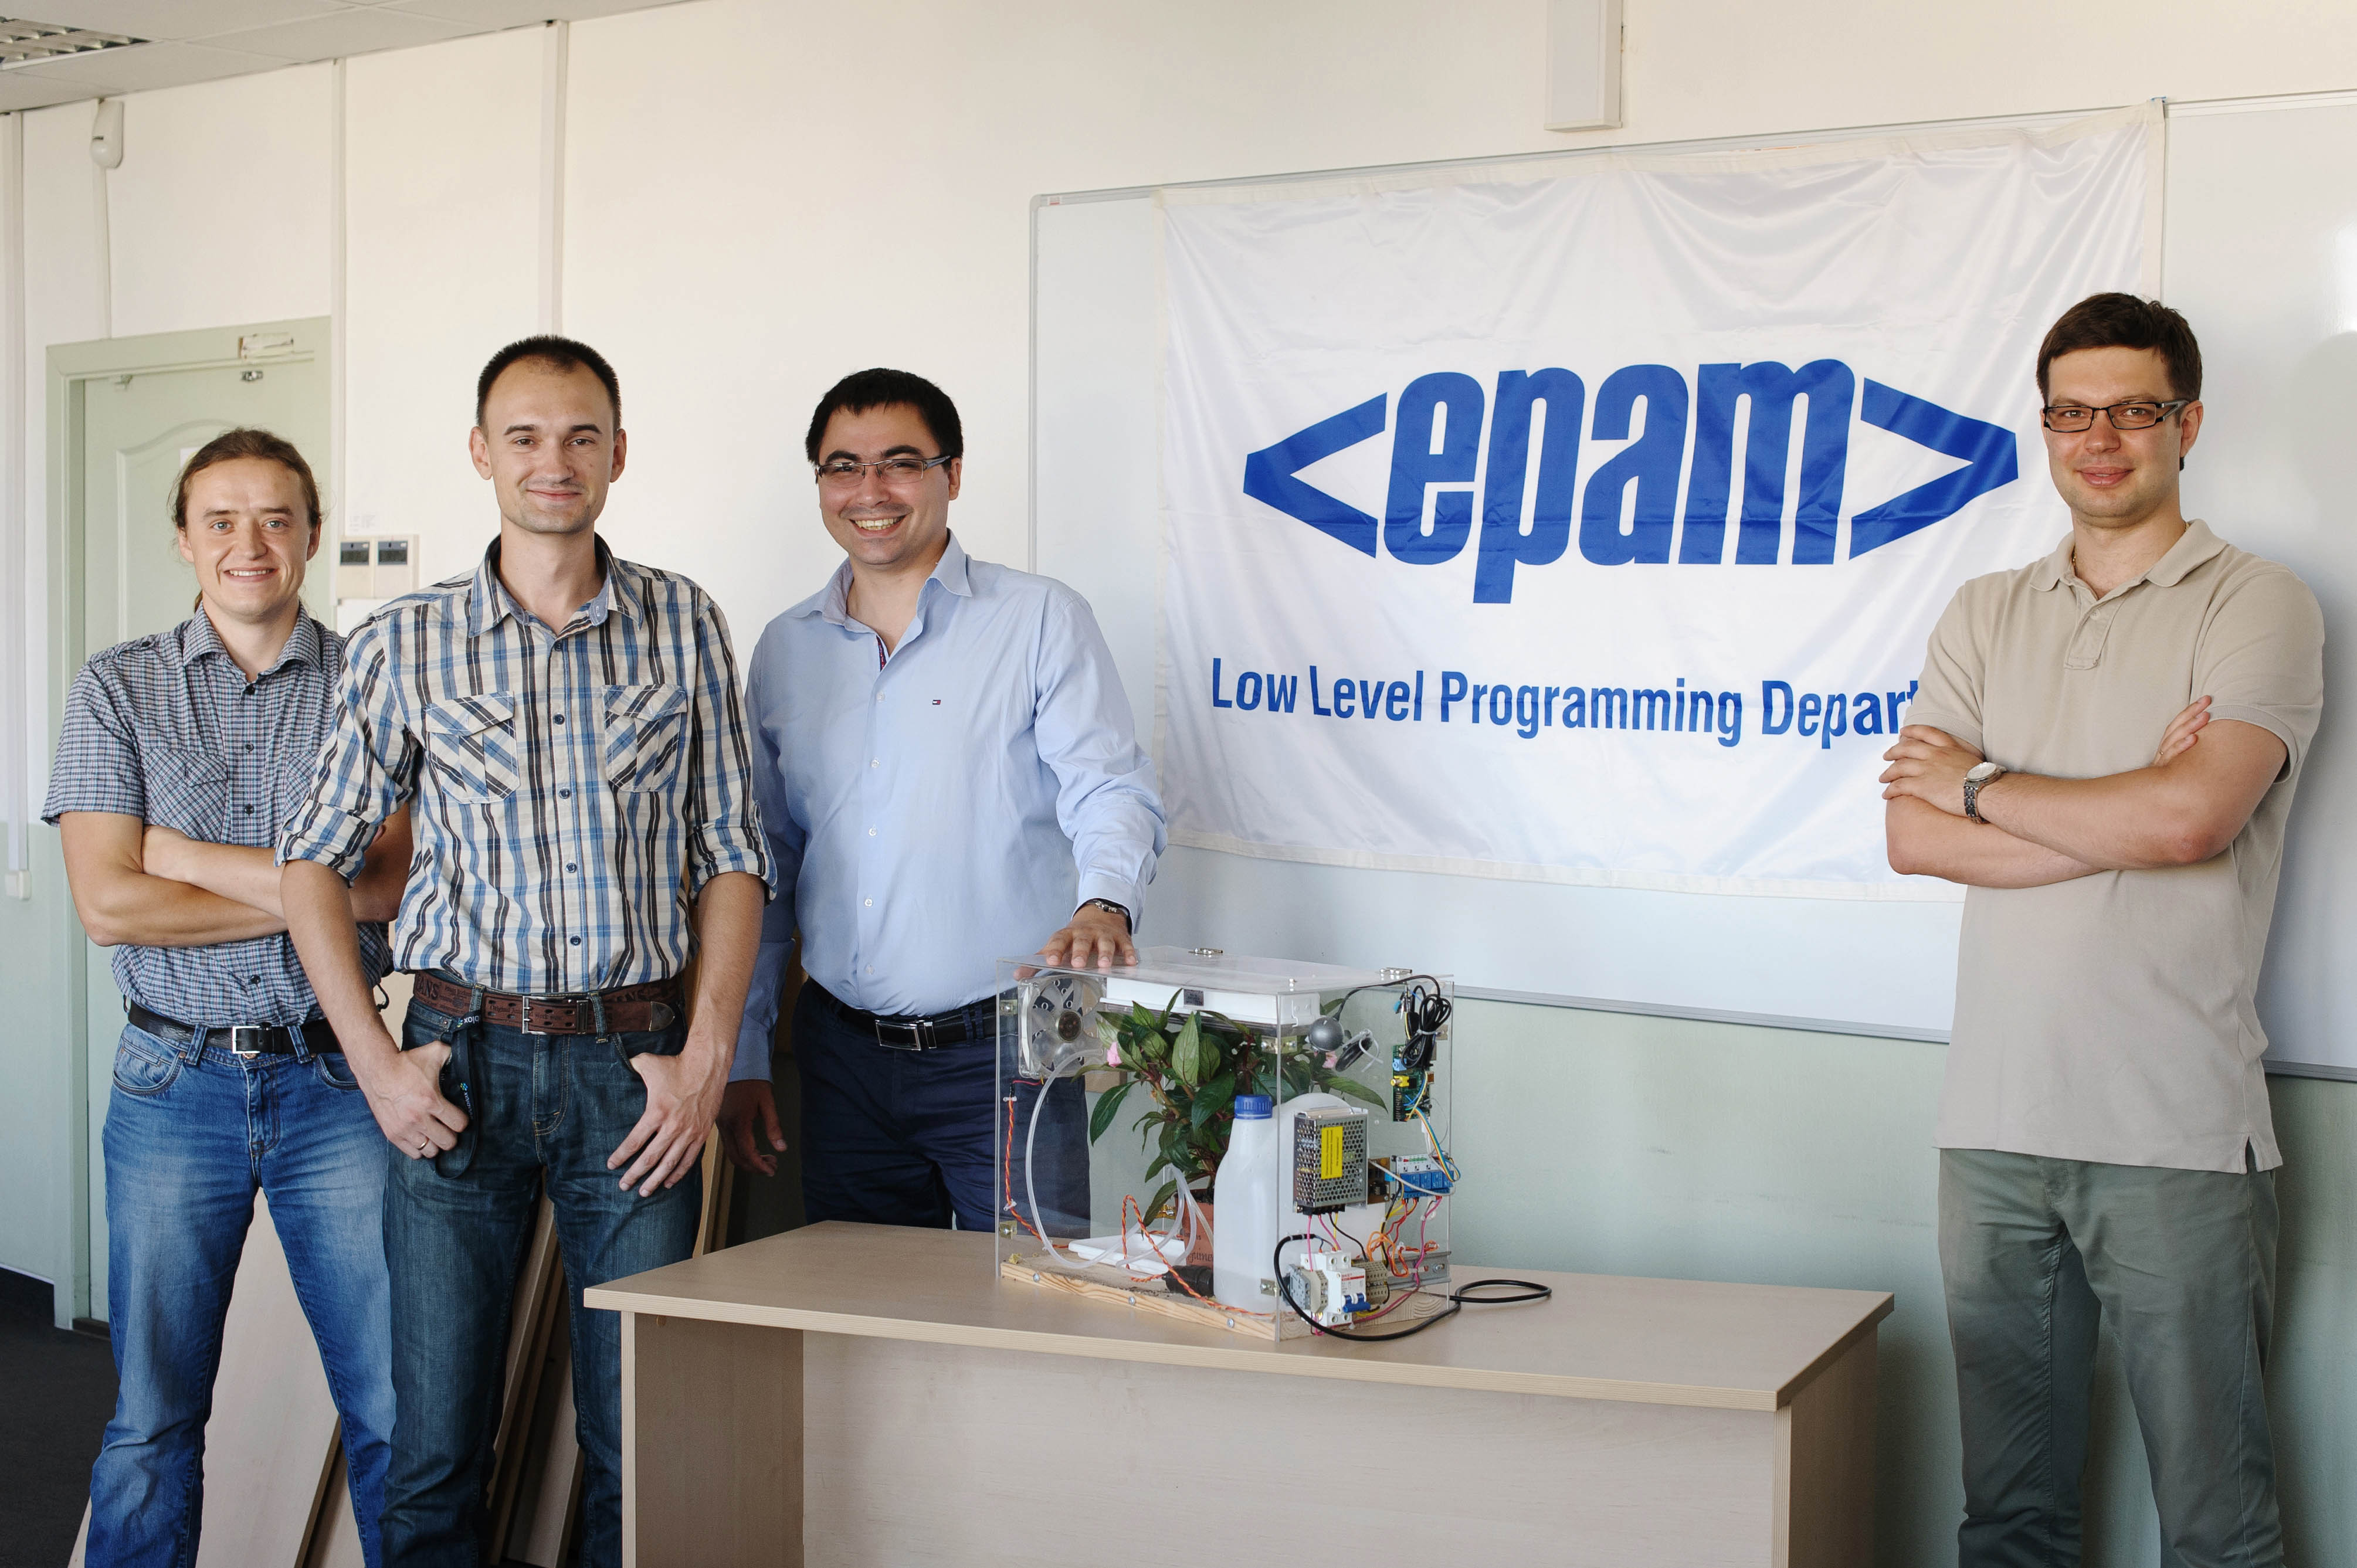
\includegraphics[scale=0.1]{Bilder/smartgreenhouse}
	\caption{Smart Greenhouse Entwicklerteam mit Miniatur-Gewächshaus\cite{i:smartgreenhouse}}
	\label{f:smartgreenhouse}
\end{figure}

Das Team begann damit, als Grundlage den Raspberry Pi festzulegen. Hiermit besaßen sie einen gut ausgestatteten Einplatinencomputer mit 700 \ac{Mhz} und 512 Mb Arbeitsspeicher, der mit 35 US\$ sehr preisgünstig ist. Doch bereits hiermit entstanden die ersten Bedenken. Um die Elektronik vor dem im Gewächshaus angebrachten Wässerungssystem zu schützen musste alles gründlich isoliert und vor eindringendem Wasser geschützt werden.\\
Da die Pi4j Bibliothek nicht die nötigen Treiber bereitstellte, die zum kommunizieren mit den Feuchtigkeitssensoren im Gewächshaus angebrachten Feuchtigkeitssensoren benötigt sind, hat das Team eigene Treiber, sowie eine Linux-basierte Betriebssystemdistribution entwickelt, die speziell auf dieses Projekt ausgerichtet ist.\\
Um dies zu ermöglichen holten sie sich die Hardwareexperten Vasili Slapik und Vladimir Redzhepov ins Team, die eine entscheidende Rolle in der Entwicklung des Projektes spielten.

Im fertiggestellten Projekt sind folgende Funktionen enthalten:\\

\begin{itemize} 
	\item Erstellung eines Belichtungsplans
	\item Erstellung eines Bewässerungsplans
	\item Temperaturkontrolle
	\item Luftfeuchtigkeitskontrolle
	\item Automatisches Management und ferngesteuerte Überwachung des Aktuellen Gewächshauszustands
	\item Automatische Erstellung eines Wachstumsverlaufs
	\item Schutz vor Überspannung / Stromausfall
\end{itemize}

Die Entwickler stellen dieses Projekt jedem Farmer kostenlos zur Verfügung. Da als Hardware nur ein Raspberry Pi sowie weitere kostengünstige Komponenten benötigt werden, kann das Smart Greenhouse von Bastlern problemlos nachgebaut werden.
Das Betriebssystem, sowie die nötige Software kann aus der Dropbox des Entwicklerteams kostenlos heruntergeladen werden.

\section{Bot-So}\label{s:Bot-So}

Das Bot-So Projekt ist ein \ac{IoT}-Roboter, der sich aus einem Raspberry Pi, Oracle Java SE Embedded 8, einem Bewegungssensor, einer Videokamera und einem Anschluss an den Kurznachrichtendienst Twitter zusammensetzt. Ziel ist es, Benutzern zu ermöglichen, ihr Zuhause oder ihre Arbeitsstelle zu überwachen, während sie selbst nicht anwesend sind. Die Kamera ist an einem Schwenkarm befestigt, der durch Rotationen einen Blickwinkel von $120^\circ$ ermöglicht. Um Sprachausgabe zu ermöglichen, besitzt der Roboter eine kleine Soundkarte, an die ein Lautsprecher angeschlossen werden kann. Dies ermöglicht das Wiedergeben von zuvor aufgenommenen Nachrichten\cite{ws:botsovoice}. Über Ethernet oder WLAN kann sich der zugrundeliegende Raspberry Pi mit dem Internet verbinden. Die für das komplette System benötigte Energie wird über USB geliefert.\\
Der Roboter kann entweder direkt angewiesen werden, einen Raum zu scannen und Videomaterial an den Besitzer zu senden, oder im Überwachungsmodus operieren. In diesem Modus  werden Bilder oder Videos aufgenommen, sobald der Bewegungssensor anschlägt\cite{z:botso}.\\

\begin{figure}[H] 
	\centering
	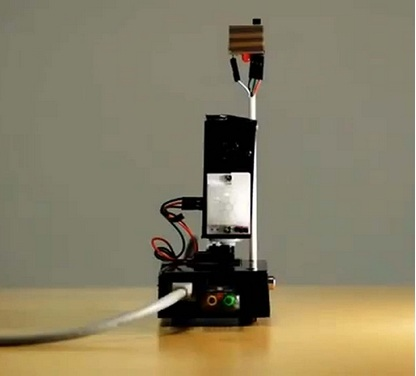
\includegraphics[scale=1.3]{Bilder/botso}
	\caption{Der Bot-So Roboter\cite{i:botso}}
	\label{f:botso}
\end{figure}

Auf dem Raspberry Pi arbeitet die weit verbreitete Debian Linux Version Raspbian, die mithilfe von Jetty, Log4j, Google Drive APIs und Java Mail die Kommunikation zum User aufnimmt. Um mit Twitter zu interagieren, bedient das Bot-So Projekt der Twitter4j Bibliothek. 

Die Kommunikation mit dem Roboter ist nahezu intuitiv. Er reagiert auf Twitter-Nachrichten wie 'Temp', woraufhin er die aktuelle Umgebungstemperatur mitteilt. 
Um einen Blick in die Umgebung des Roboters zu werfen, kann man sich entweder dem Tweet 'Take 3' bedienen, oder auf 'Sweep Room' ausweichen. Während bei 'Take 3' drei Bilder mit verschiedenen Ausrichtungen aufgezeichnet werden, fährt der Schwenkarm des Roboters bei 'Sweep Room' einmal von links nach rechts durch den Raum und zeichnet dabei ein Video auf. 
Die Dateiübertragung erfolgt über Google-Drive. Nach erfolgreichem Aufzeichnen von Video- oder Bildmaterial wird dies von dem Roboter an Google übertragen und ein Link an den Besitzer getwittert.\\


Das Robotersystem wurde von den Indern Debraj Dutta, Avinaba Brandhu Majumder, Tapas Bose und Suddhantha Krishan entwickelt. Zusammen haben sie die IoT Developer Challenge gewonnen und daraufhin die Java-One Messe besucht, um ihr Projekt vorzustellen.\\

Die Entwickler haben sich dazu entschieden, bei der Entwicklung des Projekts nur auf Open-Source Ressourcen zuzugreifen. Aufgrund dessen kann der Bot-So Roboter von jedem Bastler nachgebaut werden. Die Software hierzu kann auf Github heruntergeladen werden.

\chapter{Zusammenfassung und Fazit}\label{c:Zusammenfassung} %Label sind zum referenzieren

\section*{Zusammenfassung}
Das \ac{IoT} spielt in der sich aktuell rapide entwickelnden Welt der Informationstechnik eine entscheidende Rolle. Es lässt sich bereits heute absehen, dass diese Rolle in der Zukunft zunehmend an Bedeutung gewinnt. Besonderes Augenmerk ist hierbei auf die Sicherheit privater Daten sowie den technischen Fortschritt immer kleiner werdender System-on-a-Chip-Lösungen zu richten. Auch in der Industrie können durch innovative Projekte und intelligent vernetzte Sensoren neue Überwachungsmechanismen entwickelt werden.\\

Der geplante Umfang dieser Studienarbeit konnte aufgrund mehrerer Faktoren nicht vollständig erreicht werden. 
Oracle SunSPOT ist ein Projekt der Firma Sun, das im Jahre 2007 vorgestellt wurde. Da mittlerweile 8 Jahre vergangen sind und das System stark veraltet ist, hat sich Oracle dazu entschieden, jeglichen Support sowie Onlinehilfe zum Anfang des Jahres 2015 einzustellen. Mit dieser Entscheidung, die in Mitten der Erstellung dieser Studienarbeit getroffen wurde, beeinflusst die praktische Umsetzung in großem Umfang.\\

Die praktische Umsetzung beschränkt sich auf die Implementierung eines Einbruchssensors durch Oracle SunSPOTs. Da der Support für moderne Betriebssysteme nicht gegeben ist, war es nicht möglich, eine Erweiterung durch Desktopanwendungen zu ermöglichen. \\

Der theoretische Abschnitt der Arbeit ist in vollem Umfang umgesetzt und entspricht somit den Anforderungen an diese Arbeit.\newpage

\section*{Fazit}

Wir, die beiden Autoren, haben während der Umsetzung viele Kenntnisse erworben und unser bestehendes Wissen über Sensornetze und das \ac{IoT} erweitert. Mit dem Einsatz modernerer Sensoren wäre allerdings eine umfangreichere praktische Arbeit möglich gewesen.\\

Insgesamt sind wir mit den erarbeiteten theoretischen und praktischen Ergebnissen zufrieden und werden auch in Zukunft mit großem Interesse das Thema \ac{IoT} und dessen Weiterentwicklung im Hinblick auf Sensornetze, Raumüberwachung und Einbruchssicherung verfolgen. 
\newpage





\appendix

%%%%%%% Seitenzähler anpassen
\pagenumbering{roman}
\setcounter{page}{\theromanPagenumber}


\chapter*{Anhang}

{\huge Beispielergebnis Bedienungsanleitungen}\\

Manchmal benutzt man Worte wie Hamburgefonts, Rafgenduks oder Handgloves, um Schriften zu testen. Manchmal Sätze, die alle Buchstaben des Alphabets enthalten - man nennt diese Sätze »Pangrams«. Sehr bekannt ist dieser: The quick brown fox jumps over the lazy old dog. Oft werden in Typoblindtexte auch fremdsprachige Satzteile eingebaut (AVAIL® and Wefox™ are testing aussi la Kerning), um die Wirkung in anderen Sprachen zu testen. In Lateinisch sieht zum Beispiel fast jede Schrift gut aus. Quod erat demonstrandum. Seit 1975 fehlen in den meisten Testtexten die Zahlen, weswegen nach TypoGb. 204 § ab dem Jahr 2034 Zahlen in 86 der Texte zur Pflicht werden.
        % Anhang Einbinden
%%%%%%%%%%%%%%%%%%%%%%%%%%%%%%%%%% Literaturverzeichnis %%%%%%%%%%%%%%%%%%%%%%%%%%%%%%%%%%%%%%%%%%%%%%%%%%%%%%%%%%%%%%%%%%%%%%%%%%%%%%%%%%%%%%%%%%%%%%%%%%%%%%%%%%%%%%%%%%
\addcontentsline{toc}{chapter}{Literaturverzeichnis}
\bibliographystyle{alphadin}        % Zitierformat (deutsch für Großschreibung) [Häufigkeit] im Text
\bibliography{Literaturverzeichnis}      % Pfad des Literaturverzeichnisses


%%%%%%% Todo Liste
\newpage
\listoftodos[Notes]
%%%%%%%

\end{document}  %%%%%%%%%%%%%%%%%%%%%%%%%%%%%%%%%%%%%%%%%%%%%%%%%%%%%%%%%%%%%%%%%%%%%%%%%%%%%%%%%%%%%%%%%%%%%%%%%%%%%%%%%%%%%%%%%%%%%%%%%%%%%%%%%%%%%%%%%%%%%%%%%%%%%%%%%%
